\documentclass[a4paper,11pt]{amsart}
\usepackage[margin=1in]{geometry}
\usepackage[utf8]{inputenc} 
\usepackage[T1]{fontenc}
\usepackage{amsmath,amssymb,subcaption,graphicx,amsthm,enumitem,mathpazo,xcolor,tikz-cd, multicol,comment,url} 

\usepackage{xcolor}
\usepackage{cite}
\graphicspath{{Figures/}}
%\usepackage[backend=bibtex]{biblatex}
%\addbibresource{references_arxiv.bib}

\usepackage{amsthm, tikz-cd, multicol}
\usetikzlibrary{positioning,calc}
\tikzset{main node/.style={circle,fill=black,draw,minimum size=.25cm,inner sep=0pt},}
\setlength\parindent{0pt}

\title[On lattice path matroid polytopes]{On lattice path matroid polytopes:\\ alcoved triangulations and snake decompositions}

\author[C. Benedetti-Velásquez]{Carolina Benedetti-Velásquez}
\address{Departamento de Matemáticas, Universidad de los Andes, Bogotá, Colombia.}
\email{c.benedetti@uniandes.edu.co }

\author[K. Knauer]{Kolja Knauer}
\address{Departament de Matem\`atiques i Inform\`atica, Universitat de Barcelona, Spain, \newline LIS, Aix-Marseille Universit\'e, CNRS, and Universit\'e de Toulon, Marseille, France.}
\email{kolja.knauer@ub.edu}

\author[J. Valencia-Porras]{Jerónimo Valencia-Porras}
\address{Department of Combinatorics and Optimization, University of Waterloo, ON, Canada.}
\email{j2valenc@uwaterloo.ca}

\newtheorem{theorem}{Theorem}[section]
\newtheorem{corollary}{Corollary}[theorem]
\newtheorem{lemma}[theorem]{Lemma}
\theoremstyle{definition}
\newtheorem{definition}{Definition}[section]
\theoremstyle{definition}
\newtheorem{proposition}[theorem]{Proposition}
\theoremstyle{definition}
\newtheorem{example}[theorem]{Example}
\theoremstyle{remark}
\newtheorem*{remark}{Remark}
\theoremstyle{definition}
\newtheorem{question}{Question}
\theoremstyle{definition}
\newtheorem{conjecture}{Conjecture}

\newcommand{\Max}{\mathrm{Max}}
\newcommand{\vol}{\mathrm{Vol}}

\DeclareMathOperator{\down}{\downarrow}

\begin{document}
\maketitle

\vspace{-0.5cm}
\begin{abstract}
    We study lattice path matroid polytopes using their alcoved triangulation. We characterize Gorenstein lattice path matroid polytopes, yielding a new class of matroids satisfying the unimodality conjecture of de Loera, Haws, and K{\"o}ppe.  Further, we characterize matroids whose polytopes are order polytopes as a special class of lattice path matroids, called snakes. Finally, we give combinatorial interpretations of the volumes and $h^*$-vectors of lattice path matroids of rank $2$ based on their snake decomposition. %in the case of rank 2. %We also find recursive formulas for the volume of these polytopes.
\end{abstract}

\section{Introduction}

Matroids originally arose as a combinatorial axiomatization of the concept of independence from linear algebra. They are at the core of many branches in mathematics such as graph theory, polyhedral geometry, optimization, and algebraic geometry (see~\cite{O11,ardila2010matroid,postnikov2006total}). 

A \textit{matroid} is a pair $M = \left(E,\mathcal{B}\right)$ where $E$ is a finite set and $\mathcal{B}$ is a non-empty collection of subsets of $E$ satisfying that for all $B_1,B_2 \in \mathcal{B}$
\begin{itemize}
          \item[] if $b_1\! \in\!  B_1\! \setminus\!  B_2$, then there is $b_2\!  \in\!  B_2\! \setminus\!  B_1$ such that $B_1\! \setminus\! \{b_1\}\!  \cup\!  \{b_2\}\!  \in\!  \mathcal{B}$. 
\end{itemize}
The set $E$ usually is identified with $[n]:=\{1,\dots,n\}$ if $|E|=n$, and we refer to it as the \emph{ground set of $M$}. The elements in $\mathcal B$ are the \emph{bases} of $M$. It can be shown that each element in $\mathcal B$ has the same size, say $k$, and we say in this case that  the \emph{rank $r(M)$} of $M$ is $k$.  A matroid $M=([n],\mathcal B)$ can also be characterized geometrically via its \emph{matroid (base) polytope} $P_M$. The vertices of $P_M$ are given by $\{e_B: B\in\mathcal B\}$ where $e_B:= \sum_{i\in B}{e}_i$ and $\{e_1,\dots,e_n\}$ is the canonical basis of $\mathbb R^n$. In view of this, we sometimes think of $M$ as being $P_M$, and vice versa (see \cite{GGMS}).

\begin{figure}[htp]
    \centering
    \includegraphics[width=.6\textwidth]{polytopeclasses.pdf}
    \caption{Classes of polytopes studied in this paper.}\label{fig:polytopeclasses}
\end{figure}

Our manuscript contributes to the study of a particular class of matroids known as \emph{lattice path matroids (LPMs)}, via the study of their matroid (base) polytope. 
In order to achieve our objectives we explore LPMs in relation with other families of polytopes (see Figure \ref{fig:polytopeclasses}), so that we extract features from those other families and adapt them to LPMs. In this manuscript we only focus on matroid base polytopes, and thus we just write matroid polytopes.

LPMs were introduced in~\cite{bonin2003lattice}. Many different aspects of LPMs have been studied in the literature:  excluded minor characterizations~\cite{Bon-10}, algebraic geometric notions~\cite{Del-12,Sch-10,Sch-11}, the Tutte polynomial~\cite{bonin2003lattice,KMR18,Mor-13}, matroid quotients~\cite{BK22,DeM-07}. Also, the face structure of LPMs has been studied in~\cite{An-17,Bid-12}. 

From the combinatorial point of view, a lattice path matroid $M=([n],\mathcal B)$ of rank $k$ is such that
any $B\in\mathcal B$ can be thought as a monotone lattice path from $(0,0)$ to $(n-k,k)$ as follows: $B$ is the lattice path whose $i$-step is north if and only if $i\in B$. There are two particular bases $U$ and $L$ of $M$ such that, as lattice paths, they determine a bounded region such that all the lattice paths from $(0,0)$ to $(n-k,k)$ within this region, are in bijection with the bases of $M$. In view of this, the region determined by $U$ and $L$ is called the \emph{diagram of $M$}. Therefore, such a lattice path matroid $M$ will be denoted $M=M[U,L]$, see Figure \ref{fig:xmpl} for an example.

The class of LPMs includes the class of \emph{Schubert matroids} (set $L$ to be first all east, then all north) and \emph{uniform matroids} (the diagram is a rectangle). 
 
We say that an LPM is a \emph{snake} if its diagram does not contain $(2\times 2)$-grids. A snake $S$ is said to be \emph{inside} an LPM $M$ if $S$ has the same rank as $M$ and (the diagram of) $S$ fits inside $M$. 
If $S$ is a snake inside $M$ then $P_S\subset P_M$ and moreover, $P_M$ can be decomposed in pieces each of which is the matroid polytope of a snake in $M$ (see \cite{chatelain2011matroid}). In Figure \ref{fig:xmpl} we display the four snakes inside the given $M$, and thus $P_M$ can be decomposed into 4 matroid polytopes corresponding to each of the snakes in $M$.

\begin{figure}[htp]
    \centering
    \includegraphics[width=.3\textwidth]{xmpl.pdf} \qquad\includegraphics[width=.3\textwidth]{decomp.pdf}
    \caption{Diagram of $M=M[1246,3568]$ highlighting in bold one of its basis $B$ (left). Collection of snakes inside $M$ (right).}
    \label{fig:xmpl}
\end{figure}

\emph{Order polytopes} introduced by Stanley in \cite{Stanley1986}, are a very prominent family that has been studied extensively. An order polytope $P$ has an underlying poset whose number of linear extensions coincides with the (normalized) volume of $P$. Order polytopes as well as matroid polytopes of LPMs belong to the family of \emph{alcoved polytopes} as defined in \cite{Lam2007}. One of our initial results shows that snake polytopes are {the} intersection of matroid polytopes and order polytopes (Theorem \ref{thm:snakes-posets}). Thus, computing the volume of a snake can be thought of as counting linear extensions of a certain poset. 

Given an integer polytope $P$, that is a polytope whose vertices have integer coordinates, let $tP$ be its dilation by an integer factor of $t$. The number of integer points in $tP$ is known to be a polynomial.
%the positive integer evaluations of a polynomial. 
This polynomial, denoted $L_P(t)$, is known as the \emph{Ehrhart polynomial} of $P$ and contains a variety of information of $P$ such as its volume \cite{CCD}. In particular, the generating series of the sequence $\{ L_P(t)\}_{t\geq 0}$, known as the Ehrhart series of $P$ can be written as a rational function as 
$$
\mathrm{Ehr}_P(z):=\displaystyle\sum_{t\geq 0}L_P(t)z^t=\dfrac{h^*_0+h^*_1z+\cdots+h^*_mz^m}{(1-z)^{d+1}}.
$$
The polynomial $h^*(P):=h^*_0+h^*_1z+\cdots+h^*_mz^m$ is known as the \emph{$h^*$-polynomial of $P$}, the tuple $(h_0^*,h_1^*,\dots,h_m^*)$ is the \emph{$h^*$-vector of $P$}, and the degree of $h^*$ satisfies $m \leq \dim(P)$. Stanley's non-negativity theorem \cite{Stanley-NonNegThm} guarantees that if $P$ is an integer polytope then its $h^*$-vector has integer and nonnegative coordinates. Thus it is natural to wonder if the coefficients of $h^*$ have a combinatorial interpretation or satisfy any natural properties of integer series. %The Ehrhart polynomial of LPMs appear in~\cite{knauer2018lattice,Bid-12}.

Given an LPM we determine under which circumstances its $h^*$-vector is palindromic. That is, we determine when $h_i^*=h_{m-i}^*$, for $0\leq i\leq m$. Polytopes whose $h^*$-vector is palindromic are said to be \emph{Gorenstein}, although there are many other equivalent ways to determine if a polytope $P$ is Gorenstein. We state this result in Theorem \ref{thm:Gorenstein-LPM} using a different characterization of being Gorenstein. We point out that our characterization of being Gorenstein complements recent work from~\cite{Hibi2021,Klbl2020,LM22}.

It was conjectured by De Loera et al. \cite[Conjecture 2]{DeLoera2008} that the $h^*$-vector of any matroid polytope is unimodal. This conjecture remains wide-open and has only been proved for small matroids~\cite[Theorem 3]{DeLoera2008}, sparse paving matroids of rank $2$~\cite[Theorem 1.3]{ferroni2021ehrhart}, and certain snakes~\cite{knauer2018lattice}. 
Since alcoved Gorenstein polytopes have unimodal $h^*$-vectors~\cite{bruns2007h} we have that our Theorem \ref{thm:Gorenstein-LPM} provides us with a family of matroids for which the conjectures by De Loera et al holds true. 

On the other hand, Neggers~\cite{N78} conjectured that if $P$ is an order polytope, then its corresponding $h^*$-polynomial is real rooted and  Stanley later even conjectured a strengthening. While the Neggers-Stanley conjecture has been disproved~\cite{B04,S07}, it remains open whether the $h^*$-vector of such $P$ has the weaker property of being unimodal, see~\cite{SS21}. Our Theorem \ref{thm:snakes-posets} shows that snakes are exactly the matroids lying in the intersection of the conjecture of Neggers and Stanley and the one of De Loera et al.

We finalize our study concentrating on LPMs of rank $2$. First we give recursive formulas for the volumes of these matroid polytopes. Then, given a Schubert matroid of rank 2, we show that the coefficients of $h^*(P_M)$ counts certain permutations. This description is given in Theorem \ref{thm:h-schubert} and relies, in particular, on the fact that snakes are order polytopes as well as alcoved polytopes. Finally, we also provide a formula for the $h^*$-vector of any LPM of rank 2 in Theorem~\ref{thm:h-any-LPM}. 

This manuscript is organized as follows. In Section \ref{sec:alcoved} we provide the background needed on alcoved polytopes, triangulations, and provide an essential result on computing $h^*$-polynomials under certain circumstances.  In Section \ref{sec:snakes_fences} we introduce our building blocks from this manuscript. Namely, we define snakes as well as fences. Fences are posets whose order polytope coincides with that of a snake. Moreover we prove that snakes are the intersection of the families of matroid polytopes and order polytopes. In Section \ref{sec:gorenstein} we analyze polytopes of LPMs. We make use of known results about interior points of these polytopes as well as their hyperplane description in order to characterize LPMs that are Gorenstein. In Section \ref{sec:volumes} we provide a recursive formula for the volume of Schubert matroids of rank 2. Afterwards, we study the alcoved triangulation $\Delta$ of an LPM $M$ and understand each piece of this triangulation as a linear extension of a fence, which in turn is a permutation. Since $P_M$ can be subdivided in submatroid polytopes, each of which is the matroid polytope of a snake in $M$, we collect the simplices of the alcoved triangulation of $M$ according to the snake where each simplex comes from. This allows us to provide an orientation of the dual graph of $\Delta$ and hence we provide a combinatorial rule for the coefficients of $h^*(P_M)$ when $M$ has rank 2. Our manuscripts ends with some questions that aim to generalize the work done here for the family of positroids.

\section{Alcoved triangulations and their graphs}\label{sec:alcoved}

Let $l\in\mathbb Z$  and let $i,j\in\{0,1,\dots,n\}$. We define the hyperplane $H_{i,j}^l$ of $\mathbb R^n$ as
$$H_{i,j}^l=\left\{ x\in\mathbb{R}^n \ | \ x_i-x_j=l \right\}$$ where $x:=(x_1,x_2,\ldots,x_n)$ and we set $x_0=0$. We denote by $\mathcal A_n$ the hyperplane arrangement consisting of all such hyperplanes $H_{ij}^l$. For instance, $\mathcal A_2$ consists of all the integer translations of $x_1=0$, $x_2=0$ and $x_1-x_2=0$. 

A hyperplane $H:a_1x_1+\cdots+a_nx_n=b$ is a \emph{defining hyperplane} of a polytope $P\subseteq\mathbb R^n$ if every point in $P$ satisfies either $a_1x_1+\cdots+a_nx_n\leq b$ or $a_1x_1+\cdots+a_nx_n\geq b$. 
It is known that if $H$ is a defining hyperplane for a polytope $P$ then $H\cap P$ is a face of $P$.
 Given a defining hyperplane $H$ of a polytope $P$, we will say that $H$ is \emph{facet-defining} for $P$ if $\dim (H\cap P)=\dim P-1$. That is, the face defined by $H\cap P$ is a facet of $P$.  We say that a polytope $P\subseteq\mathbb R^n$ is an \emph{alcoved polytope} if all its facet-defining hyperplanes are of the form $H_{ij}^l$ for some $i,j,l$. It follows that  (see \cite{Lam2007}) $P$ can be described as
\begin{equation}\label{H-alcoved}P = \left\{ x\in\mathbb{R}^n \ | \ a_{ij} \leq x_i-x_j \leq b_{ij} \right\}\end{equation}
for certain collection of integers $a_{ij}$ and $b_{ij}$, where again $i,j\in\{0,1,\dots,n\}$ and $x_0=0$.

An important class of alcoved polytopes was studied by Stanley~\cite{Stanley1986}. Given a poset $X$ on $[n]$, its \textit{order polytope} $\mathcal{O}(X)$ is the set of vectors ${x}\in\mathbb{R}^n$ satisfying $0\leq x_i \leq 1$ and $x_i\geq x_j$ when $i<j$ in $X$. Hence such a polytope is alcoved. In Figure~\ref{fig:orderpoly} we provide an example.

\begin{figure}[htp]
    \centering
    \includegraphics[width=.9\textwidth]{orderpoly.pdf}
    \caption{A poset $X$, its order polytope $\mathcal{O}(X)$, its alcoved triangulation $\Delta$, and the dual graph $G_{\Delta}$.}\label{fig:orderpoly}
\end{figure}

If $P\subset\mathbb R^n$ is a polytope of dimension $d$, we refer to it as a $d$-polytope.
A \textit{triangulation} of a $d$-polytope $P$ is a set $\Delta=\{F_1,\dots,F_r\}$ of  $d$-simplices such that: \begin{itemize}
    \item the union $\bigcup_{i=1}^rF_i$ equals $P$,
    \item $F_i\cap F_j$ is a (possibly empty) face of both $F_i$ and $F_j$.
    %\item for every $i$, the vertices of $F_i$ are vertices of $P$.
\end{itemize}   
Note that in particular, the set $V$ of vertices of $\Delta$ can be a super set of the vertices of $P$. 
The arrangement $\mathcal{A}_n$ subdivides $\mathbb{R}^n$ into simplices, each of which is affinely equivalent to the unit simplex of $\mathbb{R}^n$. Thus, if $P$ is an alcoved polytope, then $\mathcal{A}_n$ induces a triangulation $\Delta$ of $P$, that is called the \emph{alcoved triangulation of $P$}, see~\cite{Lam2007}.

A triangulation of a polytope $P\subseteq \mathbb{R}^n$ is called \emph{regular} if it can be obtained by \emph{lifting} its vertices $V$ into $\mathbb {R} ^{n+1}$, i.e., adding an $(n+1)$-th coordinate to each point of $V$, computing the convex hull $H$ of the lifted set, and projecting the lower faces of $H$ back to $\mathbb {R} ^{n}$. Here a lower point of $H$ is one that minimizes the $(n+1)$-th coordinate. 

\begin{theorem}\label{sliced-triang-regular}
Let $P$ be an alcoved polytope. Then its alcoved triangulation $\Delta$ is regular.
\end{theorem}

\begin{proof}
Let $\{{n_1},\ldots,{n_k}\}$ be the normal vectors of $\mathcal{A}_n$, so that its hyperplanes are $$H_{i,j} = \left\{{x}\in\mathbb{R}^n\ | \ \langle {x},{n}_i\rangle = j\right\},$$ and consider the map $f( x)=\sum_{i=1}^k \langle {x},{n_i}  \rangle^2$. As it is a sum of convex functions, it is convex. We will use this map to lift the vertices of $\Delta$ and prove that in each cell $f$ coincides with a unique affine linear map. This suffices to show that $\Delta$ is regular. 

Let $F\in \Delta$. Since $F$ is enclosed between consecutive hyperplanes whose normal vectors are integer, for each ${n_i}$, the set of integer points in $F$ has a partition $$F \cap \mathbb{Z}^n = \left\{ {x}\in\mathbb{R}^n \ | \ \langle {x},{n_i}\rangle=k_{i, F }  \right\}\sqcup\left\{ {x}\in\mathbb{R}^n \ | \ \langle {x},{n_i}\rangle=k_{i, F }+1 \right\}$$ for some $k_{i, F }\in\mathbb{Z}$. Notice that on $F \cap \mathbb{Z}^n$ the summand $\langle {x},{n_i}  \rangle^2$ of $f$ coincides with the linear map $$g_{i, F }({x}) = (k_{i, F } +1)^2\left( \langle {x},{n_i} \rangle - k_{i, F } \right) + k_{i, F }^2\left( k_{i, F }+1- \langle {x},{n_i} \rangle \right).$$ Thus, on $ F \cap \mathbb{Z}^n$ we have $f({x})=\sum_{i=1}^{k}g_{i, F }({x})=:g_ F ({x})$. To show that each $g_{i, F }(x)$ is uniquely determined by $k_{i, F }$, consider the affine linear map $$\tilde{g}_{i, F }:\mathbb{R}^n\mathbin{/}H_{i,0} \cong \mathbb{R} \to \mathbb{R},$$ that satisfies
 $\tilde{g}_{i, F }(k_{i, F }) = k_{i, F }^2$ and $\tilde{g}_{i, F }(k_{i, F }+1)=(k_{i, F }+1)^2$. As we are specifying two values for the map it is unique, and fully determines the map $g_{i, F }(x)$ since this is constant in each $H_{i,k}$. Here we take the projection of ${n_i}$ as a basis for $\mathbb{R}^n\mathbin{/}H_{i,0}$.
 
Now, let $ F'  \neq  F $ be another cell in the subdivision. Then, the set $( F  \cup  F' )\cap\mathbb{Z}^n$ cannot be expressed as a disjoint union of two parts as before because there should be points in at least 3 hyperplanes for some direction ${n_j}$. Without loss of generality, we can assume 

\begin{align*}
    ( F  \cup  F' )\cap\mathbb{Z}^n = &\left\{ x\in\mathbb{R}^n \ | \ \langle x,n_j\rangle=k_{j}-1  \right\}\\ &\sqcup\left\{ x\in\mathbb{R}^n \ | \ \langle x,n_j\rangle=k_{j} \right\}\\ &\sqcup\left\{ x\in\mathbb{R}^n \ | \ \langle x,n_j\rangle=k_{j}+1 \right\}
\end{align*}
for some $k_j\in\mathbb{Z}$ . Suppose by contradiction that $f({x})$ coincides in $ F  \cup  F' $ with a linear affine map $h({x})$. Then, this induces an affine linear map $\tilde{h}:\mathbb{R}^n\mathbin{/}H_{i,0} \to \mathbb{R}$ such that $\tilde{h}(k_j-1)=(k_j-1)^2$, $\tilde{h}(k_j)=(k_j)^2$ and $\tilde{h}(k_j+1)=(k_j+1)^2$. However, no three points in a parabola can be joined using a line as $\tilde{h}(k)=k^2$ is a strictly convex function. Then, each cell of the subdivision has a unique affine linear map such that $f({x})$ coincides with it in the given cell. As $f({x})$ is a convex function, the convex hull of the lifted vertices (in $\mathbb{R}^{n+1}$) of the subdivision forms a polytope, whose lower faces project to the subdivision by construction. 
 
\end{proof}

Given a graph $G$ with vertex set $V_G$ and $x,y\in V_G$, we denote by $d(x,y)$ the \emph{distance} between $x$ and $y$. That is, $d(x,y)$ is the length of a shortest path between $x$ and $y$, in $G$. Given a triangulation $\Delta=\{F_1, \ldots, F_r\}$ of a polytope $P\subset\mathbb R^n$, the \textit{dual graph} $G_\Delta$ of $\Delta$ has vertex set $\Delta$ and there is an edge between two simplices $F_i, F_j$ whenever $F_i\cap F_j$ is a facet of both, $F_1$ and $F_2$. If $P$ is alcoved, notice that when $F_i\cap F_j$ is a facet of both simplices, that facet lives in a hyperplane $H\in\mathcal{A}_n$. In this case we refer to $H$ as the hyperplane \emph{generated} by $F_i\cap F_j.$
If $\Delta$ is the alcoved triangulation of an alcoved polytope $P$, then $G_{\Delta}$ can be seen as a restriction of the dual graph of the braid arrangement $\mathcal{A}_n$ to a convex region. In this setting it is known that $G_{\Delta}$ is an (isometric) subgraph of the hypercube, see~\cite{BCK18}. In particular this yields the following. 

\begin{proposition}\label{prop:alcovedgraphs}
The dual graph $G_\Delta$ of the alcoved triangulation $\Delta$ of an alcoved polytope $P$ is a connected bipartite graph and the distance $d(F,F')$ of two simplices is the number of hyperplanes of $\mathcal{A}_n$ separating them.
\end{proposition}

If $X$ is a poset on $n$ elements and $\varphi:X\to [n]$ is a bijection such that $i \leq_X j$ if and only if $\varphi(i)\leq \varphi(j)$, then $\varphi$ is called a \emph{linear extension} of $X$. The \emph{linear extension graph} $L_X$ of $X$ is the graph whose vertex set consist of all the linear extensions of $X$ and there is an edge between two vertices $\varphi$ and $\psi$ whenever there are $i,j\in X$ such that  $\varphi(i)+1=\varphi(j)=\psi(i)=\psi(j)+1$ and $\varphi(k)=\psi(k)$ for all $k\in X\setminus\{ i,j\}$. From~\cite[Section 7.2]{Lam2007} the following result is in order. See also Figure~\ref{fig:orderpoly} for an illustration.

\begin{proposition}\label{prop:linext}
If $\Delta$ is the alcoved triangulation of an order polytope $\mathcal{O}(X)$, then $G_\Delta$ is isomorphic to the linear extension graph $L_X$ of $X$.
\end{proposition}

Going back to the general setting, let $P$ be an alcoved polytope and let $\Delta$ be its alcoved triangulation. Pick an arbitrary  vertex $F_0$ of $G_{\Delta}$. We define the poset $X_\Delta(F_0)$ whose elements are the simplices in $\Delta$, by setting $F\leq F'$ if there is an  $(F_0,F')$-path in $G_{\Delta}$ that goes through $F$. Also, let $D'_{\Delta(F_0)}$ be the partial orientation of $G_{\Delta}$, where the edge between a pair of adjacent cells $F,F'$ is oriented as $(F,F')$ if $F$ and $F_0$ lie on the same side of the hyperplane generated by $F\cap F'$. 

Let $D_\Delta(F)$ be the partial orientation of $G_\Delta$, where the edge between a pair of adjacent cells $F,F'$ is oriented as $(F,F')$ if and only if $d(F_0,F') = d(F_0,F)+1$.  Otherwise, the edge is just left without orientation.


\begin{lemma}\label{lem:linext}
 If $\Delta$ is the alcoved triangulation of an alcoved polytope $P$ and $F_0\in \Delta$, then  $D'_{\Delta(F_0)}$ and $D_{\Delta(F_0)}$ coincide. Furthermore, $D'_{\Delta(F_0)}$ (and hence $D_{\Delta(F_0)}$) is the Hasse diagram of $X_\Delta(F_0)$.
\end{lemma}
\begin{proof}
 
If $(F,F')$ is an arc of $D'_{\Delta(F_0)}$ then the hyperplane $H$ generated by $F\cap F'$ has $F$ and $F_0$ on the same side. Thus, the number of hyperplanes from $\mathcal{A}_n$ separating $F$ and $F_0$ is one less than the number of hyperplanes from $\mathcal{A}_n$ separating $F'$ and $F_0$. Hence, by Proposition~\ref{prop:alcovedgraphs} we have $d(F_0,F') = d(F_0,F)+1$ and thus $(F,F')$ in $D_{\Delta(F_0)}$.

Conversely, if $(F,F')\in D_{\Delta(F_0)}$ then $d(F_0,F') = d(F_0,F)+1$. Let $H\in\mathcal{A}_n$ be the hyperplane defined by  $F\cap F'$. By the definition of $\Delta$ the hyperplane $H$ has to have $F_0$ and $F$ on the same side. Otherwise, if $F_0$ was on the same side of $H$ as $F'$ then by Proposition~\ref{prop:alcovedgraphs} we would have $d(F_0,F')+1 = d(F_0,F)$ which is a contradiction. Hence, $(F,F')\in D'_{\Delta(F_0)}$.

Finally, every cover relation of $X_\Delta(F_0)$ is achieved by an arc of $D_{\Delta(F_0)}$. Let us show that $D_{\Delta(F_0)}$ has only these arcs. On one hand, by Proposition~\ref{prop:alcovedgraphs} it holds that $G_{\Delta}$ is bipartite and $D_{\Delta(F_0)}$ has no undirected edges. On the other hand, by the definition of $D_{\Delta(F_0)}$,  any two directed paths between two vertices $F,F'$ have the same length. Hence, all arcs of $D_{\Delta(F_0)}$ correspond to cover relations.
\end{proof}

Using the notation from Lemma~\ref{lem:linext} we refer to $D_{\Delta(F_0)}$ as \emph{the orientation of $G_{\Delta}$ away from $F_0$}.

A pure simplicial complex $\Delta=\{F_1, \ldots, F_r\}$ is said to be \textit{shellable} if there is a linear ordering $\varphi:\Delta\to[r]$ such that for any $2\leq i \leq r$, $\varphi^{-1}(i)\cap\left( \varphi^{-1}(1)\cup\ldots\cup \varphi^{-1}(i-1) \right)$ is a union of facets of $\varphi^{-1}(i)$ (see \cite{braun2016shellability}). 

\begin{proposition}\label{Prop:linear-ext-are-shellings}
Let $P$ be an alcoved polytope with alcoved triangualtion $\Delta$. Fix a cell $F$ of $\Delta$, and let $\phi$ be a linear extension of the poset $X_\Delta(F)$. Then $\phi$ induces a shelling order of $\Delta$.
\end{proposition}

\begin{proof}
By Proposition~\ref{sliced-triang-regular} the triangulation $\Delta$ is regular. It is well-known that starting at any fixed cell $F$, there exists a \emph{line-shelling} $\varphi_0$ starting at $F$, i.e., $F=\varphi_0^{-1}(1)$, see~\cite[Chapter 8]{ziegler1995lectures} for more details. In \cite[Lemma 3.4]{NonCrossing} it is shown that given $\varphi_0$ orienting every edge $\{F',F''\}$ of $G_\Delta$ from $F'$ to $F''$ whenever $\varphi_0(F') < \varphi_0(F'')$, one obtains $D'_\Delta(F)$. By Lemma~\ref{lem:linext}, this implies that $\varphi_0$ is a linear extension of $X_\Delta(F)$. 

We consider the graph of linear extensions $L_{X_\Delta({F})}$ of $X_\Delta({F})$. By Proposition~\ref{prop:linext} this graph is the dual graph of the alcoved triangulation of the order polytope of $X_\Delta({F})$ and thus by Proposition~\ref{prop:alcovedgraphs} it is connected and bipartite. We prove by induction on the distance $d(\varphi_0,\varphi)$ in $L_{X_\Delta({F})}$ that every linear extension $\varphi$ of $X_\Delta({F})$ is a shelling order of $\Delta$. This is clear for $d(\varphi_0,\varphi)=0$ by the first paragraph. 

If $d(\varphi_0,\varphi)>0$, then on a shortest $(\varphi_0,\varphi)$-path the last vertex $\psi$ before $\varphi$ satsifies $d(\varphi_0,\varphi)=d(\varphi_0,\psi)+d(\psi,\varphi)$, where $d(\psi,\varphi)=1$. Hence, by induction hypothesis we have that $\psi$ is a shelling order and $\{\psi,\varphi\}$ is an edge of $L_{X_\Delta({F})}$. 
Then there exist a pair of incomparable elements, which swap from $\psi$ to obtain $\varphi$. Label the order defined by $\psi$ as $(F_1<_\psi\ldots<_\psi F_n<_\psi F_{n+1}<_\psi\ldots<_\psi F_r)$. Then the order defined by $\varphi$ is the same except for $F_{n+1}<_\varphi F_{n}$, i.e., $(F_1<_\varphi\ldots<_\varphi F_{n+1}<_\varphi F_{n}<_\varphi\ldots<_\varphi F_r)$.
In order to show that $\varphi$ is a shelling order, we make use of the fact that since both $\varphi$ and $\psi$ are linear extensions of $X_\Delta({F})$, hence, $F_{n+1},F_{n}$ are incomparable and have no edge in $G_\Delta$. Thus, the codimension of $F_{n+1}\cap F_{n}$ is larger than $1$. Since $\psi$ is a shelling order, there exists a facet of the form $F_{n+1}\cap F_{k}$ with $k<n$ such that it contains $F_n\cap F_{n+1}$. Therefore, any $x\in F_n \cap F_{n+1}$ satisfies $x\in F_n \cap F_{n+1} \cap F_{k} \subseteq F_{n} \cap F_{k}$. 


Now, in order to verify that $\varphi$ is a shelling sequence we only have to check  what happens when adding $F_{n+1}$ and afterwards $F_n$:

Let us first consider adding $F_{n+1}$ without having added $F_n$.
Note that $F_{n+1}\cap(F_1\cup\ldots\cup F_{n-1})=F_{n+1}\cap(F_1\cup\ldots\cup F_{n})\cup (F_{n+1}\cap F_{n})$. Now, since $\psi$ is a shelling order $F_{n+1}\cap(F_1\cup\ldots\cup F_{n})$ is a union of facets of $F_{n+1}$ and $F_{n+1}\cap F_{n}\subseteq F_k$ for some facet with $k<n$, we have that $F_{n+1}\cap(F_1\cup\ldots\cup F_{n-1})$ is a union of facets of $F_{n+1}$.

Let us now conisder adding $F_n$ after having added $F_{n+1}$ and note that $F_{n}\cap(F_1\cup\ldots\cup F_{n-1}\cup F_{n+1})) = F_{n}\cap( F_1\cup\ldots\cup F_{n-1}) \cup ( F_n\cap F_{n+1}).$ Similarly, since $\psi$ is a shelling order $F_{n}\cap(F_1\cup\ldots\cup F_{n-1})$ is a union of facets of $F_{n}$ and $F_{n+1}\cap F_{n}\subseteq F_k$ for some facet with $k<n$. We have that $F_{n}\cap(F_1\cup\ldots\cup F_{n-1}\cup F_{n+1}))$ is a union of facets of $F_{n}$.

This concludes the proof as the other cases follow directly from the fact that $\psi$ is a shelling order.
\end{proof}

\begin{theorem}\label{thm:h-star-and-orientations-sliced}
Let $P$ be an alcoved polytope with alcoved triangulation $\Delta$ and fix a simplex $F_0$ in $\Delta$. Consider the dual graph $G_\Delta$ of this triangulation and let $D_\Delta(F_0)$ its orientation away from $F_0$. Then $$h_k^*(P) = \#\left\{ F\in G_\Delta \;\big| \; F\text{ has }k\text{ incoming arcs in }D_\Delta(F_0) \right\}.$$
\end{theorem}

\begin{proof}
It is well-known that $\Delta$ is a \emph{unimodular}, i.e.,  $\mathrm{vol}(F_i)=1$, for each $i=1,\ldots, r$. Furthermore, $\Delta$ is shellable by Proposition \ref{Prop:linear-ext-are-shellings}. Under these conditions $$\sum_{j=0}^d h_j^*z^j = \sum_{F\in\text{max}(\Delta)}z^{n(F)}$$ where $n(F)$ is the number of simplices that intersect with $F$ in a facet and come before $F$ in the shelling order, see e.g.~\cite[Theorem 3.1]{braun2016shellability}. So far we just invoked that general theorem for unimodular, shellable triangulations. However, now we can give a more combinatorial interpretation in terms of $D_{\Delta}(F_0)$.

By Proposition \ref{Prop:linear-ext-are-shellings}, we can take a linear extension $\phi$ of $X_\Delta({F_0})$ as shelling order. Since $D_\Delta(F_0)$ is the Hasse diagram of $X_\Delta({F_0})$, for a simplex $F$ the number of simplices coming before $F$ in $\phi$ and intersecting it in a facet coincides with the number of incoming arcs of $F$ in $D_\Delta(F_0)$. This concludes the proof.
\end{proof}

Since one of our main purposes is to provide a combinatorial formula for the $h^*$-vector of certain matroid polytopes, Theorem~\ref{thm:h-star-and-orientations-sliced} will be one of the main tools to do so, once we guarantee the hypothesis needed to make use of it. This will be done in Section~\ref{sec:LPM-rank2}. 

\section{Snakes and fences}\label{sec:snakes_fences}
In this manuscript we are going to focus on (polytopes of) a very specific class of matroids known as \emph{lattice path matroids}, LPMs for short, as defined next. 


To any $k$-element subset $B\subseteq[n]:=\{1,2,\dots,n\}$ we associate a monotone lattice path from $(0,0)$ to $(n-k,k)$ whose $i$-th step is north if and only if $i\in B$. Conversely, from any such lattice path you can recover a $k$-subset of $[n]$. This correspondence will be used implicitly throughout the paper.

\begin{definition}\label{def:lpm} 

Given two lattice paths $U,L$ from $(0,0)$ to $(n-k,k)$, such that $U$ is above $L$, the \emph{lattice path matroid $M=M[U,L]$} is the matroid on $[n]$ of rank $k$ such that its bases are the set of all lattice paths from $(0,0)$ to $(n-k,k)$ inside the region enclosed by $U$ and $L$. We refer to this region as the \emph{diagram} of $M[U,L]$. 
\end{definition} 

Examples of LPMs include \emph{Schubert matroids} and \emph{uniform matroids}. An LPM $M=M[U,L]$ over $[n]$ of rank $k$ is said to be a Schubert matroid if $L$ has its last $k$ steps north. On the other hand, when the diagram of $M$ is the rectangle $(n-k,k)$, the LPM it gives rise to is known as the uniform matroid over $[n]$ of rank $k$, and it is denoted $U_{k,n}$.

We aim to understand the matroid (base) polytope $P_M$ using the analysis made in Section~\ref{sec:alcoved} when $M$ is an LPM, in particular. Thus we need to provide the necessary tools in order to use the results for alcoved polytopes. In particular, it is known that if $M$ is an LPM then its matroid polytope $P_M$ is an alcoved polytope \cite{Lam2007, knauer2018lattice}.
Our analysis of $P_M$ will show that $P_M$ can be decomposed in subpolytopes, where each subpolytope in the decomposition is the matroid polytope of \emph{snakes}. 

\begin{definition}\label{def:snakes}
Let $M=M[U,L]$ be an LPM. $M$ is said to be \emph{connected} if its diagram is connected. That is, if $U$ and $L$ only intersect in $(0,0)$ and $(n-k,k)$. A lattice path matroid $S$ is a \emph{snake} if $S$ is connected and its diagram does not contain a $2\times 2$ square. 
\end{definition}

Recall that the \emph{direct sum} $M_1\oplus M_2$ of two matroids $M_1=(E_1,\mathcal{B}_1), M_2=(E_2,\mathcal{B}_2)$ where $E_1\cap E_2=\emptyset$ is the matroid on $E_1\cup E_2$ whose set of bases is $\{B_1\cup B_2\mid B_1\in \mathcal{B}_1, B_2\in \mathcal{B}_2\}$. A matroid is \emph{connected}  if it cannot be written as the direct sum of two matroids. 
The reader can notice that Definition \ref{def:snakes} coincides with connectedness in the sense we just described. 
The direct sum of two LPMs corresponds graphically to concatenation of their corresponding diagrams, as shown in Figure~\ref{fig:LPM-direct-sum}.
\begin{figure}[ht]
    \centering
    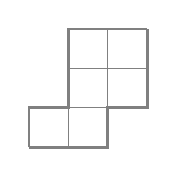
\begin{tikzpicture}
             \draw[step=0.5cm, color=gray] (0, 0) grid (1,0.5);
             \draw[step=0.5cm, color=gray] (0.5, 0.5) grid (1.5,1.5);
            \draw[line width=1pt, color = gray] (0,0) -- (0,0.5) -- (0.5,0.5) -- (0.5,1.5) -- (1.5,1.5);
            \draw[line width=1pt, color = gray] (0,0) -- (1,0) -- (1,0.5) -- (1.5,0.5) -- (1.5,1.5);
    \end{tikzpicture}
    \hspace{1cm}
    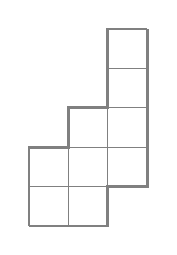
\begin{tikzpicture}
             \draw[step=0.5cm, color=gray] (0,0) grid (1,1);
             \draw[step=0.5cm, color=gray] (0.5,1) grid (1,1.5);
             \draw[step=0.5cm, color=gray] (1,0.5) grid (1.5,2.5);
            \draw[line width=1pt, color = gray] (0,0) -- (0,1) -- (0.5,1) -- (0.5,1.5) -- (1,1.5) -- (1,2.5) -- (1.5,2.5);
            \draw[line width=1pt, color = gray] (0,0) -- (1,0) -- (1,0.5) -- (1.5,0.5) -- (1.5,2.5);
    \end{tikzpicture}
    \hspace{1cm}
    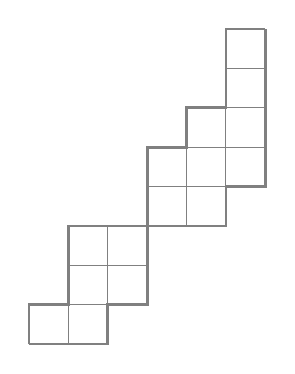
\begin{tikzpicture}
            \draw[step=0.5cm, color=gray] (0, 0) grid (1,0.5);
            \draw[step=0.5cm, color=gray] (0.5, 0.5) grid (1.5,1.5);
             \draw[step=0.5cm, color=gray] (1.5,1.5) grid (2.5,2.5);
             \draw[step=0.5cm, color=gray] (2.5, 2) grid (3,4);
             \draw[step=0.5cm, color=gray] (2,2.5) grid (2.5,3);
            \draw[line width=1pt, color = gray] (0,0) -- (0,0.5) -- (0.5,0.5) -- (0.5,1.5) -- (1.5,1.5);
            \draw[line width=1pt, color = gray] (0,0) -- (1,0) -- (1,0.5) -- (1.5,0.5) -- (1.5,1.5);
            \draw[line width=1pt, color=gray] (1.5,1.5) -- (1.5,2.5) -- (2,2.5) -- (2,3) -- (2.5,3) -- (2.5,4) -- (3,4);
            \draw[line width=1pt, color=gray] (1.5,1.5) -- (2.5,1.5) -- (2.5,2) -- (3,2) -- (3,4);
    \end{tikzpicture}
    \caption{Diagrams of two LPMs and their the direct sum.}
    \label{fig:LPM-direct-sum}
\end{figure}

Let $\alpha=(\alpha_1,\dots,\alpha_s)$ be a tuple of positive integers such that $\alpha_1+\cdots+\alpha_s=n$. That is, $\alpha$ is a \emph{composition of $n$}, denoted $\alpha\models n$. Identify each $\alpha_i$ with a rectangle $R_i$ of size $1\times (a_i+1)$, called a \emph{vertical strip}. Such $R_i$ gives rise to a \emph{horizontal strip} $R_i^*$ which is the rectangle $(a_i+1)\times 1$. Notice that $R_i$ and $R_i^*$ contain $\alpha_i+1$ unit squares.
Given a composition $\alpha=(\alpha_1,\dots,\alpha_s)$ let $S(\alpha)$ be the snake whose diagram is obtained as follows. 
From $(0,0)$ draw $R_1$, then identify its last square with the first square of $R_2^*$, then the last square of $R_2^*$ with the first square of $R_3$, and so on. On the other hand, the composition $\alpha=(\alpha_1,\dots,\alpha_s)$ gives rise to the snake $S^*(\alpha)$ obtained by reflecting $S(\alpha)$ across the line $y=x$. More precisely, $S^*(\alpha)$ is obtained as follows: From $(0,0)$ draw $R_1^*$, then identify its last square with the first square of $R_2$, then its last square with the first square of $R_3^*$, and so on. Notice that if $\alpha\models n$ then $S(\alpha)$, and hence $S^*(\alpha)$, are LPMs on the set $n+2.$ See Figure \ref{fig:snake-and-poset} for an example of a snake $S(\alpha).$ 

In this section we will conclude that matroid polytopes of snakes are exactly the matroid polytopes that are order polytopes coming from \emph{fences}. Fences are a natural class of posets that appear in the study of cluster algebras, quiver representations and other areas of enumerative combinatorics, see~\cite{MSS21} for an overview. In order to achieve this, we start by assigning a fence to a given snake $S(\alpha).$


Let $\alpha=(\alpha_1,\dots,\alpha_s)\models n$. 
The \emph{fence} of $\alpha$, denoted $F(\alpha)$ is the poset on $n+1$ elements $p_1,\ldots,p_{n+1}$ with the covering relations: 
\begin{equation*}
p_1\prec p_2 \prec \cdots\prec p_{\alpha_1+1}\succ p_{\alpha_1+2}\succ \cdots\succ p_{\alpha_1+\alpha_2+1}\prec p_{\alpha_1+\alpha_2+2}\prec\cdots\prec p_{\alpha_1+\alpha_2+\alpha_3+1}\succ \cdots.
\end{equation*}

Denote  the dual poset of $F(\alpha)$ by $F^*(\alpha)$.
Sometimes in the literature, the dual of a fence is not considered a fence, but for our purposes, both  $F(\alpha)$ and $F^*(\alpha)$ are fences. 

Given a poset $X$ we denote by $G_X$ the undirected graph obtained from the Hasse diagram of $X$, ignoring orientation of the edges. The graph $G_X$ is known as the \emph{cover graph of $X$}. Thus, a poset $X$ is a fence if its cover graph $G_X$ is a path. 

It has been shown in~\cite{knauer2018lattice} that the base polytope $P_{S(\alpha)}$ of the snake $S(\alpha)$ and the order polytope $\mathcal{O}(X)$ of the fence $F(\alpha)$ are affinely equivalent. Moreover, this result extends to direct sums of snakes and disjoint unions of fences. We describe this constructions through an example in Figure~\ref{fig:snake-and-poset}. One way of constructing the Hasse diagram of $F(\alpha)$ is to delete the first and last steps in the upper (or lower) paths defining the $S(\alpha)$ and rotating this path $45$ degrees. Note that in~\cite{knauer2018lattice}, fences were called \emph{zig-zag-chain posets}. 

\begin{figure}[ht]
    \centering
    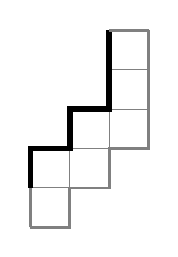
\begin{tikzpicture}
            \draw[step=0.5cm, color=gray] (0, 0) grid (0.5,1);
            \draw[step=0.5cm, color=gray] (0.5, 0.5) grid (1,1.5);
            \draw[step=0.5cm, color=gray] (1,1) grid (1.5,2.5);
            
            \draw[line width=2pt, color = black] (0,0.5) -- (0,1) -- (0.5,1) -- (0.5,1.5) -- (1,1.5) -- (1,2.5);
            \draw[line width=1pt, color=gray] (0,0) -- (0.5,0) -- (0.5,0.5) -- (1,0.5) -- (1,1) -- (1.5,1) -- (1.5,2.5);
            \draw[line width=1pt, color = gray] (0,0) -- (0,0.5);
            \draw[line width=1pt, color = gray] (1,2.5) -- (1.5,2.5);
    \end{tikzpicture}
    \hspace{2cm}
    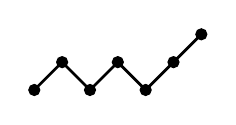
\begin{tikzpicture}[rotate = -45]
            \draw[line width=1pt] (0.5,0) -- (0.5,0.5) -- (1,0.5) -- (1,1) -- (1.5,1) -- (1.5,2); 
            
            \filldraw [color = black] (0.5,0) circle (2pt);
            \filldraw [color = black] (0.5,0.5) circle (2pt);
            \filldraw [color = black] (1,0.5) circle (2pt);
            \filldraw [color = black] (1,1) circle (2pt);
            \filldraw [color = black] (1.5,1) circle (2pt);
            \filldraw [color = black] (1.5,1.5) circle (2pt);
            \filldraw [color = black] (1.5,2) circle (2pt);
    \end{tikzpicture}
    \caption{The snake $S(1,1,1,1,2) = M[12467,24678]$ and its associated fence $F(1,1,1,1,2)$.}
    \label{fig:snake-and-poset}
\end{figure}

Before stating and proving the main result of this section we will establish a couple  of auxiliary results. We denote by $G(P)$ the 1-skeleton of a polytope $P$. That is, $G(P)$ is the graph of the polytope $P$. Also, given a poset $X$ and $x\in X$ we denote by $\down x$ the principal ideal generated by $x$. That is, $\down x:=\{y\in X : y\leq x \}$. From Stanley~\cite{Stanley1986}, we recall that every ideal $I$ of $X$ gives rise to a vertex $e_I$ of $\mathcal{O}(X)$, and every vertex of $\mathcal{O}(X)$ arises this way.

\begin{lemma}\cite[Lemma 1.1a]{HIBI2017991}\label{lemma:edges_order_polytope}
Let $I,$ be ideals of a poset $X$, with $I\neq J$. Then $\{e_I,e_J\}$ is an edge in $G(\mathcal{O}(X))$ if and only if $I\subset J$ and $J\setminus I$ induces a connected subposet of $X$.
\end{lemma}

The reader can check that Lemma~\ref{lemma:edges_order_polytope} allows one to conclude the following:

\begin{itemize}
    \item[$\circ$] if there is no containment relation between $I,J$, then vertices $e_I,e_J$ are not adjacent.
    \item[$\circ$] if $J=\down x$ for some $x\in X$ and $I\subset J$, then $\{e_I,e_J\}$ is an edge of $\mathcal{O}(X)$ since for every $y\in J\setminus I$ there is a path from $y$ to $x$, and thus $J\setminus I$ is connected. More generally, if $J=\down x\cup I$ and $x\notin I$, then $\{e_I,e_J\}$ is an edge of $\mathcal{O}(X)$.
\end{itemize}
In order to state the following lemma, found in \cite[Lemma 1.4, Lemma 1.6]{MAURER1973216}, we denote by $I(x,y)$ the \emph{interval} in $G$ corresponding to the subgraph induced by all the vertices that lie on a shortest path. In other words, $I(x,y)=\{z\in V_G\mid d(x,z)+d(z,y)=d(x,y)\}$, where $d$ is the distance function of $G$.

\begin{lemma}\label{lem:IC-PC}
    Let $M$ be a matroid and $P_M$ its matroid polytope. The following conditions hold:
    \begin{itemize}
        \item \textbf{Interval Condition (IC)}: If $x,y$ are vertices of $G(P_M)$ with $d(x,y) = 2$, then $I(x,y)$ is (isomorphic to) the graph of a square, a square pyramid or an octahedron.
        \item \textbf{Positioning Condition (PC)}: If $a,b,c,d$ are vertices that induce a square in $G(P_M)$, then for any vertex  $x$ it holds that $d(x,a) + d(x,c) = d(x,b) + d(x,d)$.
    \end{itemize}
\end{lemma}

Now we are in position to state our main result in this Section.

\begin{theorem}\label{thm:snakes-posets}
Let $P_M$ be the polytope of a connected matroid $M$. Then the following are equivalent:
\begin{enumerate}
    \item[(i)] $M$ is a snake.
    \item[(ii)] $P_M$ is affinely equivalent to an order polytope $\mathcal{O}(X)$ of a {fence} $X$. 
    \item[(iii)] $P_M$ is affinely equivalent to an order polytope $\mathcal{O}(X)$ for some poset $X$.
    \item[(iv)] The {graph} $G(P_M)$ is isomorphic to $G(\mathcal{O}(X))$ for some order polytope $\mathcal{O}(X)$.
\end{enumerate}
\end{theorem}

\begin{proof} 
Conditions (i) and (ii) are proven to be equivalent in~\cite[Theorem 4.7]{knauer2018lattice}. Also, it is clear that (ii)$\implies$ (iii) and (iii)$\implies$ (iv). %Thus, in the following we  show (iv)$\implies$ (ii).
Now we will show that (iv)$\implies$(ii).

Let $M$ be a matroid with polytope $P_M$ such that the graph $G(P_M)$ is isomorphic to $G(\mathcal{O}(X))$ for some poset $X$. In order to show that $X$ is a fence, we will show that the cover graph of $X$, $G_X$, is such that the maximum degree among all of its vertices is 2, and that $G_X$ is acyclic and connected. The proof goes by contradiction, considering different cases which we illustrate in Figure~\ref{fig:cases}.


\begin{figure}[htp]
    \centering
    \includegraphics[width=\textwidth]{snakeorder-1}
    \caption{The cases in the proof of Theorem~\ref{thm:snakes-posets}.}\label{fig:cases}
\end{figure}

As a first observation once can see that if $G_X$ has several connected components corresponding to different posets, then $\mathcal{O}(X)=P_M$ would be a product of their order polytopes. However, this would contradict that $M$ is connected. 

Now, suppose that $G_X$ has a vertex of degree larger than $2$. There are essentially two ways this can happen:

\medskip

\noindent\emph{Case 1}: There are $c,d\prec b\prec a$ in $X$ and $c,d$ are incomparable. In this case consider the four principal ideals $\down a$, $\down  b$, $\down  c$, $\down  d$, along with $\down c \cup \down d$ and $\down c \cap \down d$. Identifying the ideal $\down  x$ with its corresponding vertex in $G_X$ we can see via Lemma \ref{lemma:edges_order_polytope} that $d(\down  c,\down  d)=2$ and all these ideals belong to the interval $[\down  c,\down  d]$. However, the vertex $\down a$ has degree at least $5$. Hence, the interval $[\down  c,\down  d]$ does not induce a square, square pyramid, or octahedron. This contradicts the IC condition from~\ref{lem:IC-PC} and thus $G(\mathcal{O}(X))$ cannot be isomorphic to $G(P_M)$.

\medskip

\noindent \emph{Case 2}: 
There are $b,c,d \prec a$ in $X$ and $a,b,c$ are incomparable.

\medskip

\noindent \emph{Subcase 2.1}: $(\down c \cup\down b \cup \down d) \setminus \down c$ and $(\down c \cup\down b \cup \down d) \setminus \down d$  both induce connected subposets of $X$.

Using Lemma \ref{lemma:edges_order_polytope} we can see that $d(\down  c,\down  d)=2$ and the interval $[\down  c,\down  d]$ contains $\down a$, $\down c \cup\down b \cup \down d$, $\down  c$, $\down  d$, and further $\down c \cup \down d$, and $\down c \cap \down d$. As in the previous case the vertex $\down a$ has degree at least $5$. Hence, the interval $[\down  c,\down  d]$ does not induce a square, square pyramid, or octahedron. Again, this contradicts the IC condition and thus $G(\mathcal{O}(X))\ncong G(P_M)$.

\medskip

After possible relabeling there only remains one further subcase:
\medskip

\noindent \emph{Subcase 2.2}: 
     If $(\down c \cup\down b \cup \down d) \setminus \down b$ and $(\down c \cup\down b \cup \down d) \setminus \down c$ are disconnected then $\down c, \down c \cup\down b, \down c \cup\down b \cup \down d, \down c \cup\down d$ induce a square, using in particular the assumption that $\down c \cup\down b \cup \down d\setminus \down c$ is disconnected. Now, distances from  $\down b$ yield
    \begin{itemize}
        \item $d(\down b, \down c) = 2$ since they are non-adjacent but can be connected through $\down a$
        \item $d(\down b , \down c \cup\down b) = 1$ as they form an edge,
        \item $d(\down b, \down c \cup\down d) = 2$  since they are non-adjacent but can be connected through $\down a$, 
        \item $d(\down b, \down c \cup\down b \cup \down d) = 2$ since they are non-adjacent by assumption but can be connected through $\down a$.  
    \end{itemize} 
Altogether, this contradicts the PC condition from Lemma~\ref{lem:IC-PC}.

Note that if $X^*$ denotes the dual poset of $X$ then $G(\mathcal{O}(X))\cong G(\mathcal{O}(X^*)$. %This implies that $G_X$ cannot have any of the other two types of degree more than three vertices either\caro{no entiendo el significado de esta l\'inea}. 
Hence, the maximum degree of $G_X$ is at most $2$.

It only remains to show that $G_X$ contains no cycles. By contradiction suppose $G_X$ has a cycle, then since the maximum degree of $G_X$ is $2$, $G_X$ must be a cycle $C$. It holds that $X$ has the same number of minima and maxima and thus we distinguish three cases:

\medskip

\noindent \emph{Case A}: $X$ has exactly one maximum:
    Let $a$ be the maximum, $d$ the minimum and $b,c$ two incomparable elements such that $d \leq b,c \leq a$. Then $d(\down d, \down b\cup \down c)=2$ and the interval $I(\down a, \down b\cup \down c)$ contains the vertex $\down a$ whose degree is at least $5$ since it is adjacent to $\down d$, $\down b$, $\down c$,  $\down a\cup \down b$ and $\emptyset$. This, and the fact that all of these vertices belong to the interval $I(\down a, \down b\cup \down c)$ contradicting IC from Lemma \ref{lemma:edges_order_polytope}. 

\medskip

\noindent \emph{Case B}: $X$ has exactly two maxima:
Let $a,b$ be the maxima, and $c,d$ the minima of $X$. Then $d(\down c, \down d)=2$ and  $I(\down c, \down d)$ contains vertex $\down a\cup \down b$ whose degree is at least $5$. Indeed, $\down a\cup \down b$ is adjacent to $\down a$, $\down b$, $\down c$, $\down d$, $\emptyset$.  Again, this violates IC from Lemma \ref{lemma:edges_order_polytope}.

\medskip
\noindent \emph{Case C}: $X$ has at least three maxima:
Denote by $\mathrm{Max}(X)$ and $\mathrm{Min}(X)$ the set of maxima and minima of $X$, respectively. Let $a\in \mathrm{Max}(X)$ be a maximum and $b,c\in \mathrm{Min}(X)$ such that $b,c\leq a$. Now,  $d(\down b, \down c)=2$ and the interval $I(\down b, \down c)$ contains vertex $\bigcup_{x\in \mathrm{Max}(X)}\down x$ whose degree is at least $5$. Indeed, it is adjacent to $\down a$, $\down b$, $\down b\cup \down c$, $\down c$, $\emptyset$. This also contradicts IC from Lemma \ref{lemma:edges_order_polytope}. 
Hence, $G_X$ is acyclic and the result follows.

\end{proof}

\section{Gorenstein LPMs}\label{sec:gorenstein}

In this section we will analyze LPM polytopes in order to provide a characterization of those that are \emph{Gorenstein}, a property satisfied by some lattice polytopes. The road map to achieve this characterization will require us to provide an understanding of minors of LPMs, as well as a hyperplane description of $P_M$. %, that is an $H$-description of $P_M$.
 We start with some necessary background for this task.

\subsection{Minors of LPMs}
Deletion and contraction are well known operations that can be performed on any matroid to produce a smaller matroid. These operations may be defined as follow.

Let $M=([n],\mathcal B)$ be a matroid of rank $k$ and recall that $i\in[n]$ is a \emph{coloop} if it is in every basis, and a \emph{loop} if it is in no bases.
Let $i\in[n]$ such that $i$ is not a coloop. The \emph{deletion} of $i$ from $M$ is the matroid $M\setminus i=([n]-\{i\},\mathcal B')$ where $\mathcal B'=\{B\in\mathcal B\; :\; i\notin B\}$. Thus in this case $M\setminus i$ has rank $k$.
 Let $i\in[n]$ such that $i$ is not a loop. The \emph{contraction} of $i$ from $M$ is the matroid $M/ i=([n]-\{i\},\mathcal B'')$ where $\mathcal B''=\{B-\{i\}\; :\; B\in\mathcal B, i\in B\}$. Thus in this case $M/i$ has rank $k-1$.
If $i$ is a coloop (loop) then $M\setminus i$ (respectively $M/i$) has bases as in $\mathcal B''$ (respectively $\mathcal B'$). A \emph{minor} of a matroid $M$ is a matroid obtained from $M$ by successively deleting and contracting elements.

The family of LPMs is known to be closed under minors. That is, given an LPM $M$ it holds that any minor of $M$ is again an LPM (see ~\cite{bonin2003lattice,BONIN2006701} for details). Let us give some intuition on what deleting or contracting an element in $M$, a given LPM, looks like. This intuition will be useful to understand facets of the polytope $P_M.$

Recall that the diagram of $M[U,L]$ is completely determined by the lattice paths  $U$ and $L$. Both of these paths have labels in $[n]$, and if the rank of $M$ is $k$ then $k$ of these labels are north steps in both paths. First, observe that $i\in[n]$ is a coloop if it corresponds to a north segment that is in both $U$ and $L$ and it is a loop if it is an east segment that is in both $U$ and $L$. In both cases contraction and deletion of $i$ just corresponds to contracting the segment of the diagram.

Suppose we want to obtain the diagram of the LPM obtained from $M$ by deleting the element $i$ that is not a coloop. That is, $M\setminus i$, for some $i\in[n]$. %We describe the change of the diagram by defining the modification of $U$ and $L$. 
Start with paths $U$ and $L$ drawn bold. Then in order to obtain $M\setminus i$, a portion of $U$ and $L$ will turn dashed. The rightmost bold portions of the lattice paths $U$ and $L$ will be shifted to the right, giving us the diagram of $M\setminus i$. More precisely,
if the $i$-th step in $U$ is vertical, then dash the steps with labels $\{i,i+1,\dots,i+j \}$ where $i+j$ is the first horizontal step from $i$. If the $i$-th step in $L$ is vertical, then dash the steps $\{i,i-1,\dots,i-j \}$ where $i-j$ is horizontal and $\{i,i-1,\dots,i-j+1 \}$ are vertical in $L$.
If $i$ happens to be horizontal in $U$ (or $L$), we dash it only. Then shift to the left the right-most bold portions of $U$ and $L$, as shown in Figure \ref{fig:LPM-deletion}.

\begin{figure}[ht]
    \centering
    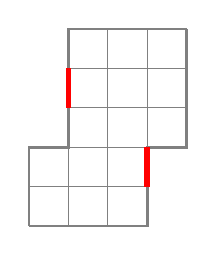
\begin{tikzpicture}
             \draw[step=0.5cm, color=gray] (0, 0) grid (1.5,1);
             \draw[step=0.5cm, color=gray] (0.5,1) grid (2,2.5);
            \draw[line width=1pt, color=gray] (0,0) -- (0,1) -- (0.5,1) -- (0.5,2.5) -- (2,2.5);
            \draw[line width=1pt, color=gray] (0,0) -- (1.5,0) -- (1.5,1) -- (2,1) -- (2,2.5);
            
            \draw[line width=2pt, color = red] (0.5,2) -- (0.5,1.5);
            \draw[line width=2pt, color = red] (1.5,1) -- (1.5,0.5);
        
    \end{tikzpicture}
    \hspace{1cm}
    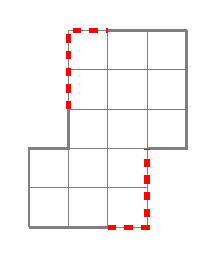
\begin{tikzpicture}
             \draw[step=0.5cm, color=gray] (0, 0) grid (1.5,1);
             \draw[step=0.5cm, color=gray] (0.5,1) grid (2,2.5);
            \draw[line width=1pt, color=gray] (0,0) -- (0,1) -- (0.5,1) -- (0.5,1.5);
            \draw[line width=1pt, color=gray] (1,2.5) -- (2,2.5);
            \draw[line width=1pt, color=gray] (0,0) -- (1,0);
            \draw[line width=1pt, color=gray] (1.5,1) -- (2,1) -- (2,2.5);
            \draw[line width=2pt, dashed,color = red] (0.5,1.5) -- (0.5,2.5) -- (1,2.5);
            \draw[line width=2pt, dashed,color = red] (1,0) -- (1.5,0) -- (1.5,1);
    \end{tikzpicture}
    \hspace{1cm}
    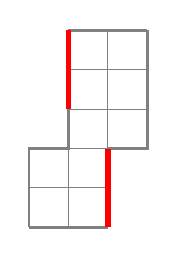
\begin{tikzpicture}
             \draw[step=0.5cm, color=gray] (0, 0) grid (1,1);
             \draw[step=0.5cm, color=gray] (0.5,1) grid (1.5,2.5);
            \draw[line width=1pt, color=gray] (0,0) -- (0,1) -- (0.5,1) -- (0.5,1.5);
            \draw[line width=1pt, color=gray] (0.5,2.5) -- (1.5,2.5);
            \draw[line width=1pt, color=gray] (0,0) -- (1,0);
            \draw[line width=1pt, color=gray] (1,1) -- (1.5,1) -- (1.5,2.5);
            \draw[line width=2pt,color = red] (0.5,1.5) -- (0.5,2.5);
            \draw[line width=2pt,color = red] (1,0) -- (1,1);
    \end{tikzpicture}
    \caption{Deletion of the element $5$ in M[12456,45789].}
    \label{fig:LPM-deletion}
\end{figure}

Now, suppose we want to contract a non-loop element $i$, and see how the contraction $M/i$ can be thought of. 
If $i$ is horizontal in $U$, then dash the steps with labels $\{i,i-1,\dots,i-j \}$ where $i-j$ is vertical and $\{i,i-1,\dots,i-j+1 \}$ are horizontal in $U$.
if $i$ is horizontal in $L$ the dash steps $\{i,i+1,\dots,i+j \}$ where $i+j$ is the first vertical step from $i$ in $L$. 
If $i$ happens to be vertical in $U$ (or $L$), we dash it only. Then shift down the upper portions of $U$ and $L$. See Figure \ref{fig:LPM-contraction} for an illustrative example.  
\begin{figure}[ht]
    \centering
    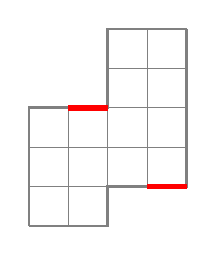
\begin{tikzpicture}
             \draw[step=0.5cm, color=gray] (0, 0) grid (1,1.5);
             \draw[step=0.5cm, color=gray] (1,0.5) grid (2,2.5);
            \draw[line width=1pt, color=gray] (0,0) -- (0,1.5) -- (1,1.5) -- (1,2.5) -- (2,2.5);
            \draw[line width=1pt, color=gray] (0,0) -- (1,0) -- (1,0.5) -- (2,0.5) -- (2,2.5);
            
            \draw[line width=2pt, color = red] (0.5,1.5) -- (1,1.5);
            \draw[line width=2pt, color = red] (2,0.5) -- (1.5,0.5);
        
    \end{tikzpicture}
    \hspace{1cm}
    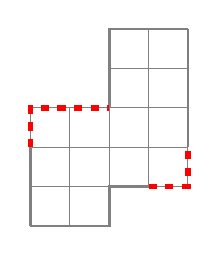
\begin{tikzpicture}
             \draw[step=0.5cm, color=gray] (0, 0) grid (1,1.5);
             \draw[step=0.5cm, color=gray] (1,0.5) grid (2,2.5);
            \draw[line width=1pt, color=gray] (0,0) -- (0,1);
            \draw[line width=1pt, color=gray] (1,1.5) -- (1,2.5) -- (2,2.5);
            \draw[line width=1pt, color=gray] (0,0) -- (1,0) -- (1,0.5) -- (1.5,0.5);
            \draw[line width=1pt, color=gray] (2,1) -- (2,2.5);
            \draw[line width=2pt, dashed, color = red] (0,1) -- (0,1.5) -- (1,1.5);
            \draw[line width=2pt, dashed, color=red] (1.5,0.5) -- (2,0.5) -- (2,1);
    \end{tikzpicture}
    \hspace{1cm}
    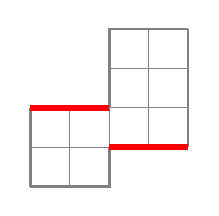
\begin{tikzpicture}
              \draw[step=0.5cm, color=gray] (0, 0) grid (1,1);
             \draw[step=0.5cm, color=gray] (1,0.5) grid (2,2);
            \draw[line width=1pt, color=gray] (0,0) -- (0,1);
            \draw[line width=1pt, color=gray] (1,1) -- (1,2) -- (2,2);
            \draw[line width=1pt, color=gray] (0,0) -- (1,0) -- (1,0.5);
            \draw[line width=1pt, color=gray] (2,0.5) -- (2,2);
            
            \draw[line width=2pt,color = red] (0,1) -- (1,1);
            \draw[line width=2pt,color = red] (1,0.5) -- (2,0.5);
    \end{tikzpicture}
    \caption{Contraction of the element $5$ in M[12367,36789].}
    \label{fig:LPM-contraction}
\end{figure}


\subsection{Face structure of LPM polytopes}
It is known that given a matroid $M$ and its polytope $P_M$, every face of $P_M$ is (the polytope of) a matroid (see \cite{GGMS}).
In this section we aim to describe these facets precisely in case that $M$ is an LPM. In particular,  we will see that the faces of $P_M$ are again LPMs. 
Given an LPM over $[n]$ of rank $k$, say $M=M[U,L]$, we have previously described $U=\{u_1,\dots,u_k\}$ by the set of labels of the $k$ north steps that define the lattice path $U$, and similar for $L$. We can also define the same lattice path $U$ as a $0/1$-vector $(U_1,U_2,\dots,U_n)$ where $U_i=1$ if and only if the $i$-th step of $U$ is north, then exactly $k$ of these $U_i$'s are equal to 1, and similar for $L$. 

With this set up in mind we establish the following result which appears in \cite[Theorem 3.3]{knauer2018lattice}, and which gives us a description of defining hyperplanes for $P_M$. 


\begin{theorem}\label{H-description-LPM-polytopes}
Let $M=M[U,L]$ be an $LPM$ of rank $k$ over $[n]$ such that $U = (U_1\ldots,U_{n})$ and $L = (L_1,\ldots,L_n)$. Then 
$$P_M = \left\{ x\in\mathbb{R}^n \;\;\; \Big| \;\;\; 0\leq x_i \leq 1 \;\; \text{and} \;\; \sum_{j=1}^{i} L_j \leq\sum_{j=1}^{i} p_j \leq \sum_{j=1}^{i} U_j \;\; \text{for all }\;i\in[n] \right\}.$$
\end{theorem}

In ~\cite[Theorem 4.1]{knauer2018lattice} the authors show that $P_M$ as given by Theorem \ref{H-description-LPM-polytopes} is affinely equivalent to a polytope $Q_M$ whose $H$-description has the form given in (\ref{H-alcoved}) which allows us to think of $P_M$ as an alcoved polytope. 

We will make use of Theorem \ref{H-description-LPM-polytopes} along with the description of minors of LPMs discussed before to describe the facet-defining hyperplanes of LPMs. Since this result is already present in the literature~\cite[Proposition 14]{An-17}, but in a slightly different set-up we only present the ideas here. Our characterization will be based on certain lattice points over the paths $U$ and $L$. Notice that the path $U$ (as well as $L$) contains $n$ lattice points, excluding $(0,0)$. The $i$-th lattice point in $U$ is the point $p_{i,U}$ with coordinates $p_{i,U}=(U_{0,i},U_{1,i})$ where $$U_{0,i}:=\displaystyle\sum_{j\leq i, U_j=0}U_j \;\;\;\text{and}\;\;\; U_{1,i}:=\displaystyle\sum_{j\leq i, U_j=1}U_j.$$ Similarly, we obtain the $i$-th lattice point $p_{i,L}$ of the lattice path $L$ as $p_{i,L}=(L_{0,i},L_{1,i})$. A \emph{point on the boundary of $M$} is a lattice point $p$ lying either on $U$ or $L$. Any point $p$ on the boundary of $M$ defines four quadrants just by translating the origin to $p$.
 We call a point $p$ on the boundary of the diagram of $M=M[U,L]$ \emph{concave} if exactly one of the four quadrants at $p$ has empty intersection with the diagram of $M$. In Figure \ref{fig:concave} the point $p=(1,2)$ of $M[12467,45678]$ is concave. 
 
 %In the case of $LPMs$ we recall that faces of LPMs are LPMs. 
 Also, if $M$ is a matroid on $n$ and $M=M_1\oplus\cdots\oplus M_r$ is its decomposition into connected components, then $\dim P_M=n-r$. Characterizing those hyperplanes in the description of $P_M$ given by Theorem \ref{H-description-LPM-polytopes}, that either correspond to a connected contraction or deletion of $M$ on one element less or to a submatroid with one more connected component yields the following: 

\begin{theorem}\label{thm:facetdefinig}
Let $M=M[U,L]$ be a connected LPM. Then the facet defining hyperplanes of $P_M$ are of the form:
\begin{itemize}
    \item[(a)] $\sum_{j=1}^{i}x_i = \sum_{j=1}^{i}L_i$ for some $1\leq i<n$ if the $i$-th point of $L$ is concave in the diagram of $M[U,L]$, or 
    \item[(b)] $\sum_{j=1}^{i}x_i = \sum_{j=1}^{i}U_i$ for some $1\leq i<n$ if the $i$-th point of $U$ is concave in the diagram of $M[U,L]$, or
    \item[(c)] $x_i=0$  for some $1\leq i\leq n$ unless the only vertical $i$-th segments among the paths in the diagram of $M[U,L]$ are the ones of $U$ and $L$, or
    \item[(d)] $x_i=1$  for some $1\leq i\leq n$  unless the only horizontal $i$-th segments among the paths in the diagram of $M[U,L]$ are the ones of $U$ and $L$.
\end{itemize}
\end{theorem}

Let us illustrate Theorem \ref{thm:facetdefinig} with an example. Consider the matroid $M=M[12467,45678]$ depicted on Figure \ref{fig:concave}. Using the notation above, the point $p=(1,2)$ being concave gives rise to the facet-defining hyperplane $H_p:x_1+x_2+x_3 = 2$. The matroid corresponding to the facet $P_M\cap H_p$ is depicted in Figure \ref{fig:concave} as well as the matroid $M_q$ corresponding to the face $P_M\cap H_{(1,3)}$, where $H_{(1,3)}:x_1+x_2+x_3+x_4 = 3$. Note that $H_{(1,3)}$, despite of being a defining hyperplane, is not a facet-defining one.


\begin{figure}[ht]
    \centering
    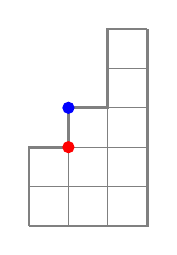
\begin{tikzpicture}
             \draw[step=0.5cm, color=gray] (0, 0) grid (1,1);
             \draw[step=0.5cm, color=gray] (1,0) grid (1.5,2.5);
             \draw[step=0.5cm, color=gray] (0.5, 1) grid (1,1.5);
             \draw[line width=1pt, color=gray] (0,0) -- (0,1) -- (0.5,1) -- (0.5,1.5) -- (1,1.5) -- (1,2.5) -- (1.5,2.5);
            \draw[line width=1pt, color=gray] (0,0) -- (1.5,0) -- (1.5,2.5);
            \filldraw [color = red] (0.5,1) circle (2pt);
            \filldraw [color = blue] (0.5,1.5) circle (2pt);
    \end{tikzpicture}
    \hspace{2cm}
    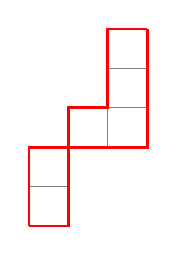
\begin{tikzpicture}
             \draw[step=0.5cm, color=gray] (0, 0) grid (0.5,1);
             \draw[step=0.5cm, color=gray] (0.5, 1) grid (1,1.5);
             \draw[step=0.5cm, color=gray] (1,1) grid (1.5,2.5);
            \draw[line width=1pt,color=red] (0,0) -- (0,1) -- (0.5,1) -- (0.5,1.5) -- (1,1.5) -- (1,2.5) -- (1.5,2.5);
            \draw[line width=1pt,color=red] (0,0) -- (0.5,0) -- (0.5,1) -- (1.5,1) -- (1.5,2.5);
    \end{tikzpicture}
    \hspace{2cm}
    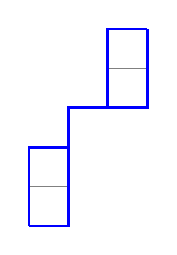
\begin{tikzpicture}
             \draw[step=0.5cm, color=gray] (0, 0) grid (0.5,1);
             \draw[step=0.5cm, color=gray] (1,1.5) grid (1.5,2.5);
            \draw[line width=1pt,color=blue] (0,0) -- (0,1) -- (0.5,1) -- (0.5,1.5) -- (1,1.5) -- (1,2.5) -- (1.5,2.5);
            \draw[line width=1pt,color=blue] (0,0) -- (0.5,0) -- (0.5,1.5) -- (1.5,1.5) -- (1.5,2.5);
    \end{tikzpicture}
        \caption{$M=M[12467,45678]$ (left), $M_{(1,2)}$ (center) and $M_{(1,3)}$ (right).}
    \label{fig:concave}
\end{figure}

\subsection{Integer and interior points of LPMs}

Let us recall some results from the literature regarding points in $P_M$ where $M$ is an LPM over $[n]$, thus $P_M\subseteq\mathbb R^n$. Given such $P_M$ we say that $Q$ is a \emph{generalized lattice path in $M$} if $Q=(s_1,\dots,s_n)$ is a sequence of $n$ line segments from $(0,0)$ to $(n-k,k)$ inside the diagram of $M$, such that the segment $s_i=\overline{AB}$ satisfies that $A=(x_{i-1},y_{i-1})$ is a point on the line $l_i=x+y=i-1$, $B=(x_{i},y_{i})\in l_{i+1}$ and $x_{i-1} \leq x_{i}$, $y_{i-1} \leq y_{i}$, for each $i\in[n]$. We refer to the tuple ${q}:=(q_1,\dots,q_n)$ as the \emph{state vector of $Q$} where $q_i$ is the slope of segment $s_i$. We will refer to the points $(x_i,y_i)$ as \emph{bending points of $Q$}. Notice that $ q$ determines $Q$ and thus we use them interchangeably. %\caro{kolja, puedes asegurarte que mi manera de reescribir esto sí corresponde a la realidad?}

In \cite{knauer2018lattice} the authors prove that $ q=(q_1,\dots,q_n)\in\mathbb R^n$ is a point in $P_M$ if and only if $ q$ is the state vector of a generalized lattice path in $M$. More concretely, they showed the following.
\begin{theorem}\cite[Theorem 3.4]{knauer2018lattice}\label{generalized-lattice-paths}
Let $M = M[U,L]$ be an LPM and $\mathcal{C}_M$ the set of state vectors of generalized lattice paths inside of the diagram of $M$. Then $P_M = \mathcal{C}_M.$
\end{theorem}

For an illustration consider Figure \ref{fig:gen-lattice-paths},  showing a generalized lattice path inside the diagram of $M=M[13,34]$, whose state vector is $\left(\frac{3}{4},0,\frac{1}{2},\frac{3}{4}\right)$.
\begin{figure}[ht]
    \centering
    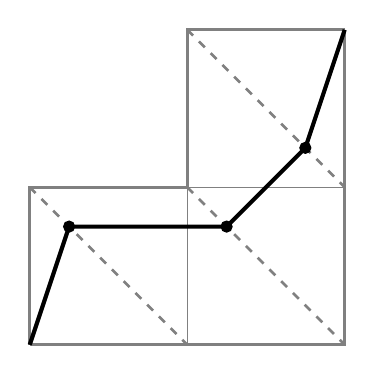
\begin{tikzpicture}
             \draw[step=2cm, color=gray] (0, 0) grid (2,2);
             \draw[step=2cm, color=gray] (2, 0) grid (4,4);
            \draw[line width=1pt, color=gray] (0,0) -- (4,0) -- (4,4);
            \draw[line width=1pt, color=gray] (0,0) -- (0,2) -- (2,2) -- (2,4) -- (4,4);
            \draw[line width = 1pt, dashed, color=gray] (0,2) -- (2,0);
            \draw[line width = 1pt, dashed, color=gray] (2,2) -- (4,0);
            \draw[line width = 1pt, dashed, color=gray] (2,4) -- (4,2);
            %\draw[line width = 1.5pt, color=blue] (0,0) -- (4,4);
            \draw[line width = 1.5pt, color=black] (0,0) -- (0.5,1.5) -- (2.5,1.5) -- (3.5,2.5) -- (4,4);
            \filldraw [color = black] (0.5,1.5) circle (2pt);
            \filldraw [color = black] (2.5,1.5) circle (2pt);
            \filldraw [color = black] (3.5,2.5) circle (2pt);
            
    \end{tikzpicture}
    \caption{A generalized lattice path in $M[13,34]$.}
    \label{fig:gen-lattice-paths}
\end{figure}


\begin{remark}\label{rem:interior_points}
Since every point in $P_M$ is a state vector $ q$ of some generalized lattice path $Q$ of $M$, then a point $p\in\mathbb R^n$ is such that $p\in tP_M\cap \mathbb Z^n$ if and only if $p=t q$ for some state vector $ q$ of $M$. The latter is equivalent to $ q$ being such that its bending points $(x_i,y_i)$ satisfy $(tx_i,ty_i)\in\mathbb Z^2$. 

We also point out that given the $H$-description of the polytope $P_M$ as in Theorem \ref{H-description-LPM-polytopes}, it follows that $p$ is in the relative interior of $P_M$, that is $p\in\text{relint} (P_M)$, if and only if $p$ is the state vector of a generalized lattice path $Q$ in $M$ such that $Q$ intersects $U$ and $L$ only in $(0,0)$ and $(n-k,k)$ and the bending points of $Q$ satisfy $x_i< x_{i+1}$ and $y_i<y_{i+1}$, for $i\in[n]$. That is, $Q$ is a strictly monotone path.
\end{remark}

\subsection{Characterizing Gorenstein LPMs}
Finally after few more definitions we will be able to state the main result of this section.
A lattice polytope $P\subset\mathbb R^n$  containing $0$ in its interior is called \textit{reflexive} if its dual (polar) polytope is also a lattice polytope. In general, one says that a lattice polytope $P$ is reflexive if a translation of it, say $P-z $ for some $z\in \mathbb R^n$, is reflexive. If $P$ is a lattice polytope we say that $P$ is \textit{($\delta$-)Gorenstein} if $\delta P$ is reflexive, for some $\delta\in\mathbb{Z}_{>0}$. %We say that $P$ is a \textit{Gorenstein polytope } if it is $\delta$-Gorenstein for some $\delta$. 
We say that a matroid $M$ is \emph{Gorenstein} if $P_M$ is Gorenstein. We encourage the reader to look at \cite{CCD} for equivalent definitions of Gorenstein, including the one we appeal to in the Introduction. 

\begin{proposition}\cite{CCD}\label{reflexive-hyperplanes}
A polytope $P$ is reflexive if and only if for every facet-defining subspace $H$ there is no integer point in $\text{aff}(P)$ between $H$ and its homogenization $H_0$.
\end{proposition}

With these concepts in mind we now establish the main result in this section.

\begin{theorem}\label{thm:Gorenstein-LPM}
Let $M = M[U,L]$ be a connected LPM over $[n]$ of rank $k$. Then $M$ is $\delta$-Gorenstein if and only if one of the following conditions holds:
\begin{enumerate}
    \item[$\delta = 2$:] the line $\ell$\,:\,$y=x$ intersects $U$ and $L$ trivially. That is $\ell\cap U\subset \{(0,0),(n-k,k)\}$ and $\ell\cap L\subset \{(0,0),(n-k,k)\}$. Additionally, every concave point $p$ in the boundary of $M$ is of the form $(i,i+1)$ or $(i+1,i)$ for some $i$.
    \item[$\delta \geq 3$:] $M$ is isomorphic to the snake $S(\delta-2,\ldots,\delta-2)$ or $S^*(\delta-2,\ldots,\delta-2)$.
\end{enumerate} 
\end{theorem} 

\begin{proof}
In order to prove this result we point out the following. If  $M = M[U,L]$ is a connected LPM which is $\delta$-Gorenstein then $\delta\geq 2$ since $P_M$ is a $0/1$-polytope. This is equivalent to the existence of some
 ${z} \in \text{relint}(\delta P)$ such that the polytope $Q := \delta P - {z}$ is reflexive. In view of the remark following Theorem \ref{generalized-lattice-paths}, ${z}$ corresponds to a strictly monotone path inside the diagram of $M$, as described in the remark. Denote this path by $\tilde z$.

From Theorem \ref{thm:facetdefinig}, there are two types of defining hyperplanes for $Q$. The ones corresponding to concave boundary points are of the form $\sum_{j=1}^i \left( \delta L_j - z_j \right) = \sum_{j=1}^i x_j$ and $\sum_{j=1}^i \left( \delta U_j - z_j \right) = \sum_{j=1}^i x_j$. The homogenization of these hyperplanes is $\sum_{j=1}^i x_j = 0$. By Proposition \ref{reflexive-hyperplanes} $M$ being Gorenstein is equivalent to the fact that there is no integer point ${p}$ in between the hyperplane and its homogenization. This means that we cannot have $\sum_{j=1}^i \left( \delta L_j - z_j \right) < \sum_{j=1}^i p_i < 0$. Therefore, $\sum_{j=1}^i \left( \delta L_j - z_j \right) = -1$ and similarly, $\sum_{j=1}^i \left( \delta U_j - z_j \right) = 1$. Equivalently, these equations are $\sum_{j=1}^i \left(L_j - \tilde{z_j}\right) = -\frac{1}{\delta}$ and $\sum_{j=1}^i \left( U_j - \tilde{z_j} \right) = \frac{1}{\delta}$ in terms of the coordinates of the lattice path $\tilde z$ corresponding to $z$. Recall that the sum from $i=1$ to $i=j$ of the coordinates of a path correspond to their height along the diagonals $x+y=k$ for $k\in\mathbb{Z}_+$ measured from the $x$ axis after placing the diagram of the LPM at the origin. 
Then these equations imply that $z$ correspond to a generalized lattice path passing $1/\delta$-units above any concave corner in $L$ and $1/\delta$-units below any concave corner in $U$. %We will consider the general case in what follows.

Now, again by Theorem~\ref{thm:facetdefinig} the contraction/deletion type of hyperplanes are of the form $0 -z_k= x_k$ or $\delta - z_k=x_k$. Using Proposition \ref{reflexive-hyperplanes} as before, we find that $z_k = 1$ or $\delta - z_k = 1$. Therefore, if the diagram has an interior point both equations must be satisfied, and this implies $\delta = 2$. The only point in $2(P-\partial P)$ is the diagonal path, and together with the condition described before, we obtain  the first part of the characterization. 

If the diagram of the matroid has no interior point, it corresponds to a snake. By Theorem~\ref{thm:facetdefinig}, in the horizontal parts of the snake only deletions are admissible, thus the path corresponding to ${z}$ has only $1/\delta$ North steps. Similarly, for the vertical parts the path has only $(\delta-1)/\delta$ North steps. Together with the condition on the concave corners of the paths, this is equivalent to the snake being isomorphic to either $S(\delta-2,\ldots,\delta-2)$ or $S^*(\delta-2,\ldots,\delta-2)$. The result follows. 
\end{proof}

\begin{figure}[ht]
    \centering
    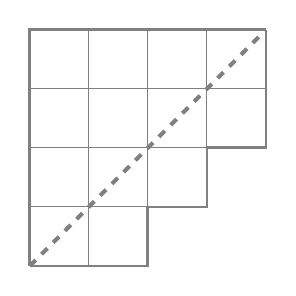
\begin{tikzpicture}
            \draw[step=0.75cm, color=gray] (0, 0) grid (1.5,3);
            \draw[step=0.75cm, color=gray] (1.5, 0.75) grid (2.25,3);
            \draw[step=0.75cm, color=gray] (2.25,1.5) grid (3,3);
           \draw[line width=1pt, color=gray] (0,0) -- (0,3) -- (3,3);
           \draw[line width=1pt, color=gray] (0,0) -- (1.5,0) -- (1.5,0.75) -- (2.25,0.75) -- (2.25,1.5) -- (3,1.5) -- (3,3);
           \draw[line width=1.5pt, dashed, color = gray] (0,0) -- (3,3);
   \end{tikzpicture}
   \hspace{0.5cm}
   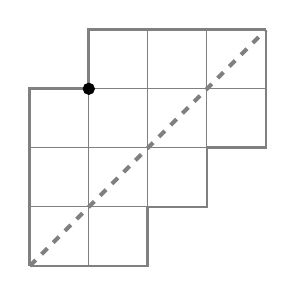
\begin{tikzpicture}
            \draw[step=0.75cm, color=gray] (0, 0) grid (1.5,2.25);
            \draw[step=0.75cm, color=gray] (1.5, 0.75) grid (2.25,3);
            \draw[step=0.75cm, color=gray] (2.25,1.5) grid (3,3);
           \draw[line width=1pt, color = gray] (0,0) -- (0,2.25) -- (0.75,2.25) -- (0.75,3) -- (3,3);
           \draw[line width=1pt, color = gray] (0,0) -- (1.5,0) -- (1.5,0.75) -- (2.25,0.75) -- (2.25,1.5) -- (3,1.5) -- (3,3);
           \draw[line width=1.5pt, dashed, color = gray] (0,0) -- (3,3);
           \filldraw [color = black] (0.75,2.25) circle (2pt);
           
   \end{tikzpicture}
   \hspace{0.5cm}
   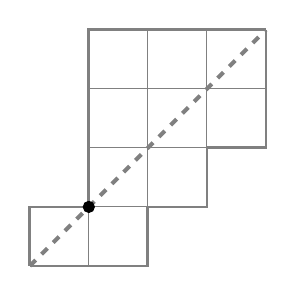
\begin{tikzpicture}
            \draw[step=0.75cm, color=gray] (0.75, 0) grid (1.5,3);
            \draw[step=0.75cm, color=gray] (1.5, 0.75) grid (2.25,3);
            \draw[step=0.75cm, color=gray] (2.25,1.5) grid (3,3);
           \draw[line width=1pt, color = gray] (0,0) -- (0,0.75) -- (0.75,0.75) -- (0.75,3) -- (3,3);
           \draw[line width=1pt, color = gray] (0,0) -- (1.5,0) -- (1.5,0.75) -- (2.25,0.75) -- (2.25,1.5) -- (3,1.5) -- (3,3);
           
           \draw[line width=1.5pt, dashed, color = gray] (0,0) -- (3,3);
           \filldraw [color = black] (0.75,0.75) circle (2pt);
   \end{tikzpicture}
    \caption{On the left an LPM satisfying condition 1. of Theorem~\ref{thm:Gorenstein-LPM}. The other two LPMs are not Gorenstein as the highlighted concave points show.}
    \label{fig:Gorenstein_LPMs}
\end{figure}

As uniform matroids are LPMs, we recover a result of \cite[Theorem 2.4]{DENEGRI1997629}.

\begin{corollary}
A uniform matroid is Gorenstein if and only if it is $U_{n,2n}$, $U_{1,n}$ or $U_{n-1,n}$. 
\end{corollary}

Finally, and as a main connection to the theme of the paper we obtain:

\begin{corollary}
If an LPM satisfies the conditions of Theorem~\ref{thm:Gorenstein-LPM}, then its $h^*$-vector is unimodal.
\end{corollary}
\begin{proof}
Let $M$ be an LPM. Since the alcoved triangulation of $P_M$ is unimodal and regular, see~\ref{sliced-triang-regular}, one can apply the results of~\cite[Theorem 1]{bruns2007h}, which guarantees that Gorenstein polytopes with such triangulations have unimodal $h^*$-vector.
\end{proof}

\section{Volumes of LPM Polytopes of rank $2$}\label{sec:volumes}


In the present section we restrict ourselves to connected LPMs. Given an LPM over $[n]$, say $M=M[U,L]$, we denote by $\mathcal{S}[U,L]$ the set of snakes over $[n]$ that fit inside the diagram of $M$. That is, snakes over $[n]$ whose boundary paths lie between $U$ and $L$. In Figure~\ref{fig:xmpl} we illustrate the snakes in $\mathcal S[1246,3568]$. A very useful property of snakes is that the set $\mathcal{S}[U,L]$ yields a decomposition of $P_M$.  More precisely,~\cite[Corollary 4]{chatelain2011matroid} gives us the following.
\begin{theorem}\label{thm:splitting}
Let $M=M[U,L]$ be an LPM over $[n]$ and let $\mathcal{S}[U,L]$ as before. We have $$P_M=\bigcup_{S\in \mathcal{S}[U,L]}P_S$$
such that $P_S\cap P_{S'}$ is a face of both $P_S,P_{S'}$ for any two distinct $S,S'\in \mathcal{S}[U,L]$.
\end{theorem}

A particular consequence of Theorem~\ref{thm:splitting} that has been used for instance in~\cite{Bid-12} is:
\begin{corollary}\label{cor:volume}
Let $M=M[U,L]$ an LPM and $\mathcal{S}[U,L]$ the set of connected snakes fitting in the diagram of $M$. We have $$\vol(P_M)=\sum_{S\in \mathcal{S}[U,L]}\vol(P_S).$$
\end{corollary}

Since our purpose in this section is to understand combinatorially the volume of (base polytopes of) LPMs of rank 2, we point out the following. Corollary \ref{cor:volume} tells us that if $M=M[U,L]$, then computing the volume of $P_M$ can be achieved by computing the volume of each $S\in \mathcal{S}[U,L]$, and then add them up. On the other hand, for each 
such $S$ we know from Theorem \ref{thm:snakes-posets} that $P_S$ is an order polytope, and its volume is the number of linear extensions of the corresponding fence $F(\alpha)$, where $S=S(\alpha)$ for some composition $\alpha$.
Now, let us illustrate a way of thinking of a linear extension of $F(\alpha)$ via a labelling of (the cells of) $S(\alpha)$. Let $\alpha\models m$ and let $S=S(\alpha)$. A \emph{labelling} $\mathcal L$ of $S$ is a labelling of its $m+1$ cells using numbers from $[m+1]$ in such a way that labels increase in each column from bottom to top and in each row from right to left. This increasing condition simply reflects the ordering of the corresponding elements in the poset $F(\alpha)$. Such labelling $\mathcal L$ induces a linear extension $\mathcal L_F$ of $F(\alpha)$ as follows: if box $i$ of $S$ has label $j$ then $p_i$ is in the $j$-th position in $\mathcal L_F$, and we write $\mathcal L_F(p_i)=j$. Here we think of $S(\alpha)$ sequentially obtained by adding first $\alpha_1+1$ boxes, then $\alpha_2$ and so on (as described in Section \ref{sec:snakes_fences}), and thus the $i$-th box of $S(\alpha)$ is the $i$-th box added in this fashion. 

\begin{example}
Let $\alpha=(1,1,1,1,2)\models 6$. In  Figure~\ref{fig:diagrams-linear-exts} we illustrate $F(\alpha)$ along with a labelling $\mathcal L$ of $S(\alpha)$. The linear extension $\mathcal L_F$ of $F(\alpha)$ induced by $\mathcal L$ 
 is $p_1 < p_5 < p_3 < p_6 < p_4 < p_7 < p_2$.

\end{example}
 
\begin{figure}[ht]
    \centering

    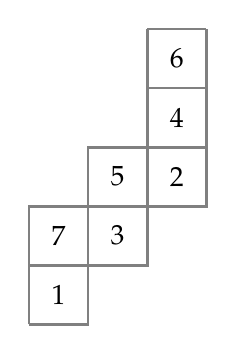
\begin{tikzpicture}[]
            \draw[line width=1pt, color = gray] (0,0.75) -- (0.75,0.75);
            \draw[line width=1pt, color = gray] (0.75,0.75) -- (0.75,1.5);
            \draw[line width=1pt, color = gray] (0.75,1.5) -- (1.5,1.5);
            \draw[line width=1pt, color = gray] (1.5,1.5) -- (1.5,2.25);
            \draw[line width=1pt, color = gray] (1.5,2.25) -- (2.25,2.25);
            \draw[line width=1pt, color = gray] (1.5,3) -- (2.25,3);
            \draw[line width=1pt, color = gray] (0,0.75) -- (0,1.5) -- (0.75,1.5) -- (0.75,2.25) -- (1.5,2.25) -- (1.5,3.75);
            \draw[line width=1pt, color=gray] (0,0) -- (0.75,0) -- (0.75,0.75) -- (1.5,0.75) -- (1.5,1.5) -- (2.25,1.5) -- (2.25,3.75);
            \draw[line width=1pt, color = gray] (0,0) -- (0,0.75);
            \draw[line width=1pt, color = gray] (1.5,3.75) -- (2.25,3.75);
            %Nodes
            \node[color = black] at (0.375,0.375) {1};
            \node[color = black] at (0.375,1.125) {7};
            \node[color = black] at (1.125,1.125) {3};
            \node[color = black] at (1.125,1.875) {5};
            \node[color = black] at (1.875,1.875) {2};
            \node[color = black] at (1.875,2.625) {4};
            \node[color = black] at (1.875,3.375) {6};
    \end{tikzpicture}
        \hspace{2cm}
    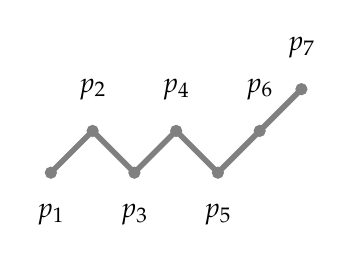
\begin{tikzpicture}[rotate = -45]
            \draw[line width=2pt, color=gray] (0.75,0) -- (0.75,0.75) -- (1.5,0.75) -- (1.5,1.5) -- (2.25,1.5) -- (2.25,3); 
            
            \filldraw [color = gray] (0.75,0) circle (2pt);
            \filldraw [color = gray] (0.75,0.75) circle (2pt);
            \filldraw [color = gray] (1.5,0.75) circle (2pt);
            \filldraw [color = gray] (1.5,1.5) circle (2pt);
            \filldraw [color = gray] (2.25,1.5) circle (2pt);
            \filldraw [color = gray] (2.25,2.25) circle (2pt);
            \filldraw [color = gray] (2.25,3) circle (2pt);
            %Nodes
            \node[color = black] at (1.125,-0.375) {$p_1$};
            \node[color = black] at (0.375,1.125) {$p_2$};
            \node[color = black] at (1.875,0.375) {$p_3$};
            \node[color = black] at (1.125,1.875) {$p_4$};
            \node[color = black] at (2.625,1.125) {$p_5$};
            \node[color = black] at (1.875,2.625) {$p_6$};
            \node[color = black] at (1.875,3.375) {$p_7$};
    \end{tikzpicture}
    
    \caption{The linear extension $p_1 < p_5 < p_3 < p_6 < p_4 < p_7 < p_2$ of $F(1,1,1,1,2)$ displayed inside the diagram of $S(1,1,1,1,2)$.}
    \label{fig:diagrams-linear-exts}
\end{figure}

\bigskip

\begin{remark}
The reader can check that this correspondence from labellings $\mathcal L$ of $S(\alpha)$ and linear extensions $\mathcal L_F$ of $F(\alpha)$ is actually a bijection. This will become relevant to us, since we will compute volumes of LPMs of rank 2, in particular, by counting linear extensions of snakes.
\end{remark}

From now on we restrict to the case of LPMs of rank 2. We introduce the following notation for such LPMs.

\begin{definition}
For all $n\geq 4$ and $1\leq k\leq \ell\leq n-2$, denote by $M_{n}[k,\ell]$ the LPM of rank 2 $M[U,L]$ where $U=\{1,n-\ell \}$  and $L=\{n-k+1,n\}$.
\end{definition}

\begin{remark}
With $k,\ell$ as before the following observations are in order:
\begin{itemize}
\item The \emph{uniform matroid of rank 2 over $[n]$}, denoted $U_{2,n}$, corresponds to $M_n[1,n-2]$.
    \item The diagram of the rank 2 matroid $M_n[k,\ell]$ is a subdiagram of that of the uniform matroid $U_{2,n}$. That is, removing the leftmost $n-2-\ell$ cells from the top row of $U_{2,n}$ and the rightmost $k-1$ cells from the bottom row of $U_{2,n}$ provides us the diagram of $M_n[k,\ell]$ (see Figure \ref{fig:schubert-notation}).
    \item \emph{Schubert matroids} are a subclass of LPMs. In particular, Schubert matroids over $[n]$ of rank 2 are obtained as $M_n[1,\ell]$, for any $1\leq \ell\leq n-2$.
    \item When $k=\ell$ the matroid $M_n[k,k]$ is a snake, denoted $S_{k,n}$, and
    $$S_{k,n}=\begin{cases}
S^*(n-3,1) & k=1\\
S^*(n-k-2,1,k-1) & 1<k<n-2 \\
S(1,n-3) & k=n-2\\
\end{cases}.
$$
\end{itemize}

\end{remark}


\begin{figure}[t]
    \centering
    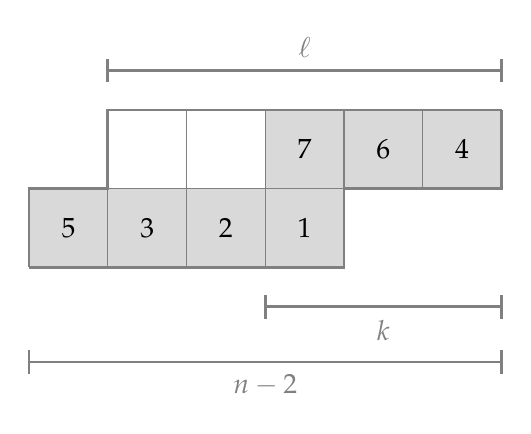
\begin{tikzpicture}            
            \filldraw[color=gray!30] (0,0) -- (0,1) -- (3,1) -- (3,2) -- (6,2) -- (6,1) -- (4,1) -- (4,0) -- (0,0);
            \draw[step=1cm, color=gray] (0, 0) grid (1,1);
            \draw[step=1cm, color=gray] (1,0) grid (4,2);
            \draw[step=1cm, color=gray] (4,1) grid (6,2);
            \draw[line width = 1pt, color=gray] (0,0) -- (0,1) -- (1,1) -- (1,2) -- (6,2);
            \draw[line width = 1pt, color=gray] (0,0) -- (4,0) -- (4,1) -- (6,1) -- (6,2);
            \draw[line width = 1pt, color=gray] (1,2.5) -- (6,2.5);
            \draw[line width = 1pt, color=gray] (3,-0.5) -- (6,-0.5);
            \draw[line width = 1pt, color=gray] (0,-1.2) -- (6,-1.2);
            \draw[line width = 1pt, color=gray] (1,2.35) -- (1,2.65);
            \draw[line width = 1pt, color=gray] (6,2.35) -- (6,2.65);
            \draw[line width = 1pt, color=gray] (3,-0.35) -- (3,-0.65);
            \draw[line width = 1pt, color=gray] (6,-0.35) -- (6,-0.65);
            \draw[line width = 1pt, color=gray] (0,-1.35) -- (0,-1.05);
            \draw[line width = 1pt, color=gray] (6,-1.35) -- (6,-1.05);
            \node[color = gray] at (3.5,2.8) {$\ell$};
            \node[color = gray] at (4.5,-0.8) {$k$};
            \node[color = gray] at (3,-1.5) {$n-2$};

            \node[color = black] at (0.5,0.5) {5};
            \node[color = black] at (1.5,0.5) {3};
            \node[color = black] at (2.5,0.5) {2};
            \node[color = black] at (3.5,0.5) {1};
            \node[color = black] at (3.5,1.5) {7};
            \node[color = black] at (4.5,1.5) {6};
            \node[color = black] at (5.5,1.5) {4};
\end{tikzpicture}
    \caption{Diagram of $M_n[k,\ell]$ where $n=8$, $k=3$ and $\ell = 5$. The snake $M_8[3,3]$ is shaded and the labelling $(A_1,A_2) = (1235,467)$ is included inside the snake.}
    \label{fig:schubert-notation}
\end{figure}

%For rank 2 LPMs, the set of snakes fitting inside of their diagram is particularly simple. We denote by  


With these observations in mind let $\sigma_n(k,\ell)$ denote the normalized volume of $M_n[k,\ell]$, for $n\geq 4$ and $0\leq k\leq \ell\leq n-2$. Otherwise set  $\sigma_n\big(k,\ell\big)=0$. 

\begin{example}
   Considering again $M=M_8[3,5]$ as in Figure \ref{fig:schubert-notation}, the set of snakes inside the diagram of $M$ is $\{S_{3,8},S_{4,8},S_{5,8}\}$. Thus, Theorem \ref{thm:splitting} tells us that $P_M$ can be decomposed into 3 matroid polytopes, each one corresponding to the given snakes inside $M$. Hence, Corollary \ref{cor:volume} tells us that $\sigma_8(3,5)=\sigma_8(3,3)+\sigma_8(4,4)+\sigma_8(5,5)$. Now, in order to compute, say, $\sigma_8(3,3)$ we need to compute the number of labellings $\mathcal L$ of this snake. Any such $\mathcal L$ gives rise to a set partition $(A_1,A_2)$ of $[8-1]$ such that $\max A_2>\min A_1$ and $|A_2|=k=3$. For instance, $(1235,467)$ is depicted in Figure \ref{fig:schubert-notation}. 
\end{example}


\begin{theorem}\label{thm:sigma-k-properties}
Let $n\geq 4$ and let $1\leq k\leq \ell\leq n-2$. Then $\sigma_n\big(k,\ell\big)$ satisfies:
\begin{enumerate}
    \item $\sigma_n\big(k,k\big) = \binom{n-1}{k} - 1$.
    \item $\sigma_n\big(k,\ell-1\big) + \sigma_n\big(k,\ell\big) + \big( \binom{n-1}{k-1} + \ell - k \big) = \sigma_{n+1}\big(k,\ell\big)$.
    \item For fixed $k$ and $\ell$, $\sigma_n\big(k,\ell\big)$ is a polynomial in $n$ of degree $\ell.$
\end{enumerate}
\end{theorem}

\begin{proof}

(1): As mentioned before, in this case $\sigma_n(k,k)$ coincides with the number of set partitions $(A_1,A_2)$ of $[n-1]$ such that $\max A_2>\min A_1$ and $|A_2|=k$. Hence, $A_2$ can be any of the $k$-subsets of $[n-1]$ except for $\{1,2,\ldots,k\}$. Hence, $\sigma_n\big(k,k\big) = \binom{n-1}{k} - 1$.

(2): We show that the set of labellings of the snakes in $M_{n+1}[k,\ell]$ can be partitioned into three disjoint sets $X_1,X_2,X_3$ where $|X_1|=\sigma_n\big(k,\ell-1\big)$, $|X_2|=\sigma_n\big(k,\ell\big)$ and $|X_3|= \binom{n-1}{k-1}+(\ell-k)$.

Let $S_{i,n+1}$ be a snake in $M_{n+1}
[k,\ell]$, then $n-2-\ell\leq i\leq n-2-k$. Let $(A_1,A_2)$ be the set partition corresponding to a labelling of $S_{i,n+1}$, as before. 
\begin{itemize}
    \item[$\circ$] Let $i< n-2-k$ and consider $S_{i,n+1}$ as before. If $n\in A_2$ then $A_2=\{a_1<\cdots<a_i=n \}$. If $\min A_1<a_{i-1}$, delete the box in $S_{i,n+2}$ labelled $n$ and push the bottom row $S_{i,n+2}$ to the right to obtain a snake in $M_n[k,\ell-1]$ whose labelling is given by $(A_2-\{n\},A_1)$. This accounts for the set $X_1$. If $\min A_1>a_{i-1}$ it implies that $A_2=\{1,\cdots,j,n\}$, and considering such labellings for each $i$ we obtain $\ell-k$ of them, giving rise to a subset of $X_3$.
    \item[$\circ$] If $i=n-2-k$, the snake $S_{i,n+1}$ is the farthest one to the right in $M_{n+1}[k,\ell]$. If $n\in A_2$ then the number of such labellings is ${{n-1}\choose{k-1}}$, accounting for the rest of $X_3$. 
    \item[$\circ$] If $n\in A_1$, deleting it gives rise to a labelling of a snake inside $M_n[k,\ell]$, and every such labellings of snakes in  arise $M_n[k,\ell]$ like this. This provides us the set $X_2$.
\end{itemize}

Finally, the polynomiality claimed in (3) follows from \cite[Prop. 1.9.2a]{EC1}.


\end{proof}

Let $A_{j,m}$ be the \emph{Eulerian number} which counts the number of permutations of the set $[m]$ with $j$-descents for $0\leq j\leq m-1$.
Notice that, for $1\leq k\leq n-2$ it holds that a labelling of the snake $S_{n-k+1,n}=(k-1,1,n-k-2)$ corresponds to a unique permutation on $[n-1]$ with only one descent. More precisely, consider the following bijection between the set $\mathcal L(S_{n-k+1,n})$ of labellings of $S_{n-k+1,n}$ and the set $D_{n-k-2,n-1}$ of permutations of $[n-1]$ (in one-line notation) with a unique descent in position $n-k-2$:

\begin{align*}
   \varphi_k:\;\;\quad\quad\quad\quad \mathcal L(S_{n-k+1,n})\quad\quad\quad\quad &\longrightarrow\quad\quad\quad\quad\;\; D_{n-k-2,n-1}\\
    \begin{matrix}
     & & & a_{k+1} & \ldots & a_{n-1}\\
    a_1 & a_2 & \ldots & a_k & & \\
    \end{matrix} \hspace{0.3cm}&\longmapsto  \hspace{0.3cm} a_{n-1} a_{n-2} \ldots a_{k+1} | a_k a_{k-1}\ldots a_1 
\end{align*}

\noindent where the vertical line in the permutation marks its unique descent. It is known that the volume of $P_M$ where $M=U_{2,n}$ is the Eulerian number $A_{1,n-1}$  (see \cite{Laplace1886}). We have therefore the following.


\begin{corollary}\label{cor:sigma-properties}
The following recursion holds for the volume of Schubert matroids of rank 2.
\begin{equation}\label{eq:sigma_recursion}
\sigma_n\big(1,\ell-1\big) + \sigma_n\big(1,\ell\big) + \ell = \sigma_{n+1}\big(1,\ell\big)
\end{equation}
where $\sigma_n\big(1,1\big) = n-2$ for every $n\geq 3$. Moreover for each $1\leq \ell\leq n-3$ one has that $A_{1,n-1} = \sigma_n(1,\ell) + \sigma_n(1,n-\ell-2)$.
\end{corollary}

\begin{proof}
The first part of the statement follows directly from Theorem \ref{thm:sigma-k-properties}. 
For the second part, for a fixed $\ell\in[n-3]$ denote by $D_{\leq \ell}$ the set of permutations of $[n-1]$ with a unique descent in position $j$ where $j\leq \ell$, and similarly $D_{\geq \ell}$. Then $|A_{1,n-1}|=|D_{\leq \ell}|+|D_{> \ell}|$. In addition, one has that $|D_{\leq \ell}|=\sigma_n(1,\ell)$ is the volume of the Schubert matroid $M_n[1,\ell]$. On the other hand the set $D_{> \ell}$ is in bijective correspondence with the labellings of snakes inside $M_n[1,n-2-\ell]$. 
\end{proof}

We refer the to OEIS sequence \url{A347976} where we display the triangle of values that Corollary \ref{cor:sigma-properties} makes allusion to.

We can extend $\sigma_n\big(1,\ell\big)$ to a function $f_\ell:\mathbb{Z} \to\mathbb{Z}$ defined by $f_\ell(n) = \sigma_n\big(1,\ell\big)$ using the recursion (\ref{eq:sigma_recursion}) from above. Below we computed $f_\ell(n)$ for $0\leq n \leq 10$ and $1\leq \ell \leq 8$ where the first column corresponds to the values of $\sigma_n\big(1,1\big)$ and the bold diagonal is the sequence $A_{1,n-1}$.  In particular, the second part of Corollary \ref{cor:sigma-properties} says for instance, that $A_{1,5}=26=22+4=\sigma_6(1,3)+\sigma_6(1,1)$.
$$
\begin{array}{c||cccccccc}
\textcolor{red}{n}\backslash \textcolor{red}{\ell} &\textcolor{red}{1} & \textcolor{red}{2} & \textcolor{red}{3} & \textcolor{red}{4} & \textcolor{red}{5} & \textcolor{red}{6} & \textcolor{red}{7} & \textcolor{red}{8} \\
\hline
\hline
\textcolor{red}{0}&\textcolor{black}{-2} & -2 & -4 & -4 & -6 & -8 & 0 & -28 \\
\textcolor{red}{1}&\textcolor{black}{-1} & -2 & -3 & -4 & -5 & -8 & -1 & -20 \\
\textcolor{red}{2}&\textcolor{black}{0} & -1 & -2 & -3 & -4 & -7 & -2 & -13 \\
\textcolor{red}{3}&\textit{\textbf{1}} & 1 & 0 & -1 & -2 & -5 & -2 & -7\\
\textcolor{red}{4}&\textcolor{black}{2} & \textit{\textbf{4}} & 4 & 3 & 2 & 1 & 0 &  -1\\
\textcolor{red}{5}&\textcolor{black}{3} & 8 & \textit{\textbf{11}} & 11 & 10 & 9 & 8 & 7 \\
\textcolor{red}{6}&\textcolor{black}{4} & 13 & 22 & \textit{\textbf{26}} & 26 & 25 & 24 & 23\\
\textcolor{red}{7}&\textcolor{black}{5} & 19 & 38 & 52 & \textit{\textbf{57}} & 57 & 56 & 55 \\
\textcolor{red}{8}&\textcolor{black}{6} & 26 & 60 & 94 & 114 &\textit{ \textbf{120}} & 120 & 119\\
\textcolor{red}{9}&\textcolor{black}{7} & 34 & 89 & 158 & 213 & 240 & \textit{\textbf{247}} & 247\\
\textcolor{red}{10}&\textcolor{black}{8} & 43 & 126 & 251 & 376 & 459 & 494 & \textit{\textbf{502}}
\end{array}
$$

With the understanding we have gained about labellings of snakes and the volume of LPMs, we will aim next to give an interpretation of the $h^*$-vector of LPMs of rank 2.

\section{The $h^*$-vector of LPMs of rank 2}\label{sec:LPM-rank2}
In \cite{Stanley1986} Stanley provided a triangulation of the uniform matroid $M=U_{k,n}$. On the other hand, in \cite{Lam2007} the authors proved that Stanley's triangulation is the alcoved triangulation of $P_{M}$. In our case, if $M$ is an LPM we will construct a triangulation $\Delta$ of $P_M$ such that $\Delta$ is obtained from Stanley's, and hence $\Delta$ is alcoved. 
The main result of this section, given in Theorem \ref{thm:h-any-LPM}, provides a combinatorial way to compute the $h^*$-vector of a $M=M[U,L]$ of rank 2. This result will be achieved in four main steps: 
\begin{enumerate}
\item We make use of Theorem \ref{thm:splitting}, which allows us to subdivide $P_M$ into pieces indexed by its set of snakes $\mathcal S [U,L]$. Next, we make use of the results relating snakes and order polytopes in Section \ref{sec:snakes_fences} in order to describe the dual graph of the alcoved triangulation of $P_M$, see Theorem~\ref{thm:dual-graph-alcoved-triangulation-LPMs}.
\item  We provide a new combinatorial interpretation for $h^*(U_{2,n})$. The coefficients of $h^*(U_{k,n})$ appeared previously in \cite[Corollary 2.9]{katzman2005hilbert} and have been given a different combinatorial interpretation in \cite{kim2020combinatorial}. However, unlike these known interpretations, ours is purely combinatorial. See Theorem~\ref{thm:h-star-permutations}.
\item We extend the interpretation of $h^*(U_{2,n})$ to Schubert matroids of rank 2, see Theorem~\ref{thm:h-schubert}.
\item We show how to obtain the $h^*$-vector of an \emph{opposite} Schubert matroid from the   $h^*$-vector of a Schubert matroid. Combining the two, we obtain an combinatorial interpretation for the $h^*$-vector of arbitrary LPMs of rank 2, see Theorem \ref{thm:h-any-LPM}.
\end{enumerate}


\subsection{Dual graph of the alcoved triangulation of an LPM}

Now we wish to describe the dual graph of the alcoved triangulation for LPMs, starting with the particular case of snakes. By Theorem~\ref{thm:snakes-posets}, matroid polytopes of snakes are order polytopes of fences. 
That is, given a snake $S$ there is a fence $F$ whose order polytope $\mathcal O(F)$ is affinely equivalent to $P_S$. The triangulation of $\mathcal O(F)$ is such that each simplex is index by a linear ordering of $F$. Thus we now want to describe what is the simplex $\Delta(\mathcal L)$ corresponding to a labelling $\mathcal L$ of the snake $S$. 

Let $S=M[U,L]$ be a snake on $[n]$, let $\mathcal{L}$ be a labelling of it and let $(L_1,\dots,L_n)$ be the state vector of $L$. Notice that the smallest label of $\mathcal L$, namely 1, appears in a position $i$ such that $L_{i-1}=0$ and $L_i=1$. We denote by $f(L)$ the \emph{flip} of the $0/1$-vector $(L_1,\dots,L_n)$ to be $$f(L) = (L_1,\dots,L_{i-2},L_i,L_{i-1},L_{i+1},\dots,L_n).$$ That is, we flip the entry $i$ where the smallest label appear, with the entry $i-1$. Remark that $f(L)$ is the state vector of another basis $B$ of $S$. %, and it now corresponds to the labelling $\mathcal L$ with the label $1$ removed. This partial labelling now has 2 (the lowest label) in position $j$, and we apply the flip map that switches positions $j-1,j$ of $B$. 
Continuing this way, $f^2(L)=f(B)$ is the state vector of another basis. % and it corresponds to  the labelling $\mathcal L$ with the labels $1,2$ removed. 
Notice also that one obtains (the state vector of) $U$ through $f^{n-1}(L)$. 
Then the simplex $\Delta(\mathcal{L})$ corresponding to $\mathcal L$ is given by
\[ \Delta(\mathcal{L}) = \text{conv}\{B_1,B_2,\dots,B_n \}\]
where each $B_i\in\mathbb R^n$ is obtained successively as follows:
\begin{itemize}
    \item[(i)] Set $B_1:=(L_1,\dots,L_n)$ to be the state vector of $L$.
    \item[(ii)] For $2\leq i\leq n$ let $B_i:=f(B_{i-1})$. 
\end{itemize}

\begin{example}  Let $S=M[14,45]$ and let $\mathcal L=(134,2)$ be a labelling of the snake.
The simplex $\Delta(\mathcal{L})$ is the convex hull of $B_1=(0,0,0,1,1)$, $B_2=(0,0,1,0,1)$, $B_3=(0,0,1,1,0)$, $B_4=(0,1,0,1,0)$ and $B_5=(1,0,0,1,0)$. Figure \ref{fig:flips} illustrates step by step the vertices of $\Delta(\mathcal{L})$ along with each basis. 

\begin{figure}[ht]
    \centering
    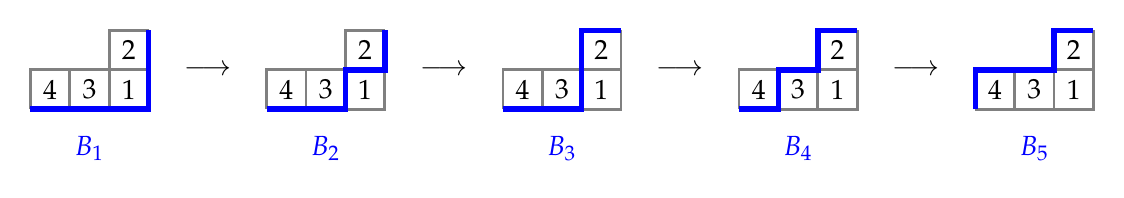
\begin{tikzpicture}
    \centering
    %Paths
        \draw[line width=1pt, color = gray] ($(0.5,0)+(0,0)$) -- ($(0.5,0.5)+(0,0)$);
        \draw[line width=1pt, color = gray] ($(1,0)+(0,0)$) -- ($(1,0.75)+(0,0)$);
        \draw[line width=1pt, color = gray] ($(1,0.5)+(0,0)$) -- ($(1.5,0.5)+(0,0)$);
        \draw[line width=1pt, color = gray] ($(0,0)+(0,0)$) -- ($(0,0.5)+(0,0)$) -- ($(1,0.5)+(0,0)$) -- ($(1,1)+(0,0)$) -- ($(1.5,1)+(0,0)$);
        \draw[line width=1pt, color = gray] ($(0,0)+(0,0)$) -- ($(1.5,0)+(0,0)$) -- ($(1.5,1)+(0,0)$);
    %Numbers
        \node[color = black] at ($(0.25,0.25)+(0,0)$) {4};
        \node[color = black] at ($(0.75,0.25)+(0,0)$) {3};
        \node[color = black] at ($(1.25,0.25)+(0,0)$) {1};
        \node[color = black] at ($(1.25,0.75)+(0,0)$) {2};
    %B_i
        \draw[line width=2pt, color = blue] ($(0,0)+(0,0)$) -- ($(1.5,0)+(0,0)$) -- ($(1.5,1)+(0,0)$);
    %Arrow
        \node[color = black] at ($(2.25,0.5)+(0,0)$) {$\longrightarrow$};
    %Label
        \node[color = blue] at ($(0.75,-0.5)+(0,0)$) {$B_1$};

    %Paths
        \draw[line width=1pt, color = gray] ($(0.5,0)+(3,0)$) -- ($(0.5,0.5)+(3,0)$);
        \draw[line width=1pt, color = gray] ($(1,0)+(3,0)$) -- ($(1,0.75)+(3,0)$);
        \draw[line width=1pt, color = gray] ($(1,0.5)+(3,0)$) -- ($(1.5,0.5)+(3,0)$);
        \draw[line width=1pt, color = gray] ($(0,0)+(3,0)$) -- ($(0,0.5)+(3,0)$) -- ($(1,0.5)+(3,0)$) -- ($(1,1)+(3,0)$) -- ($(1.5,1)+(3,0)$);
        \draw[line width=1pt, color = gray] ($(0,0)+(3,0)$) -- ($(1.5,0)+(3,0)$) -- ($(1.5,1)+(3,0)$);
    %Numbers
        \node[color = black] at ($(0.25,0.25)+(3,0)$) {4};
        \node[color = black] at ($(0.75,0.25)+(3,0)$) {3};
        \node[color = black] at ($(1.25,0.25)+(3,0)$) {1};
        \node[color = black] at ($(1.25,0.75)+(3,0)$) {2};
    %B_i
        \draw[line width=2pt, color = blue] ($(0,0)+(3,0)$) -- ($(1.0,0)+(3,0)$) -- ($(1,0.5)+(3,0)$) -- ($(1.5,0.5)+(3,0)$) -- ($(1.5,1)+(3,0)$);
    %Arrow
        \node[color = black] at ($(2.25,0.5)+(3,0)$) {$\longrightarrow$};
    %Label
        \node[color = blue] at ($(0.75,-0.5)+(3,0)$) {$B_2$};

    %Paths
        \draw[line width=1pt, color = gray] ($(0.5,0)+(6,0)$) -- ($(0.5,0.5)+(6,0)$);
        \draw[line width=1pt, color = gray] ($(1,0)+(6,0)$) -- ($(1,0.75)+(6,0)$);
        \draw[line width=1pt, color = gray] ($(1,0.5)+(6,0)$) -- ($(1.5,0.5)+(6,0)$);
        \draw[line width=1pt, color = gray] ($(0,0)+(6,0)$) -- ($(0,0.5)+(6,0)$) -- ($(1,0.5)+(6,0)$) -- ($(1,1)+(6,0)$) -- ($(1.5,1)+(6,0)$);
        \draw[line width=1pt, color = gray] ($(0,0)+(6,0)$) -- ($(1.5,0)+(6,0)$) -- ($(1.5,1)+(6,0)$);
    %Numbers
        \node[color = black] at ($(0.25,0.25)+(6,0)$) {4};
        \node[color = black] at ($(0.75,0.25)+(6,0)$) {3};
        \node[color = black] at ($(1.25,0.25)+(6,0)$) {1};
        \node[color = black] at ($(1.25,0.75)+(6,0)$) {2};
    %B_i
        \draw[line width=2pt, color = blue] ($(0,0)+(6,0)$) -- ($(1,0)+(6,0)$) -- ($(1,1)+(6,0)$)  -- ($(1.5,1)+(6,0)$);
    %Arrow
        \node[color = black] at ($(2.25,0.5)+(6,0)$) {$\longrightarrow$};
    %Label
        \node[color = blue] at ($(0.75,-0.5)+(6,0)$) {$B_3$};

    %Paths
        \draw[line width=1pt, color = gray] ($(0.5,0)+(9,0)$) -- ($(0.5,0.5)+(9,0)$);
        \draw[line width=1pt, color = gray] ($(1,0)+(9,0)$) -- ($(1,0.75)+(9,0)$);
        \draw[line width=1pt, color = gray] ($(1,0.5)+(9,0)$) -- ($(1.5,0.5)+(9,0)$);
        \draw[line width=1pt, color = gray] ($(0,0)+(9,0)$) -- ($(0,0.5)+(9,0)$) -- ($(1,0.5)+(9,0)$) -- ($(1,1)+(9,0)$) -- ($(1.5,1)+(9,0)$);
        \draw[line width=1pt, color = gray] ($(0,0)+(9,0)$) -- ($(1.5,0)+(9,0)$) -- ($(1.5,1)+(9,0)$);
    %Numbers
        \node[color = black] at ($(0.25,0.25)+(9,0)$) {4};
        \node[color = black] at ($(0.75,0.25)+(9,0)$) {3};
        \node[color = black] at ($(1.25,0.25)+(9,0)$) {1};
        \node[color = black] at ($(1.25,0.75)+(9,0)$) {2};
    %B_i
        \draw[line width=2pt, color = blue] ($(0,0)+(9,0)$) -- ($(0.5,0)+(9,0)$) -- ($(0.5,0.5)+(9,0)$) -- ($(1,0.5)+(9,0)$) -- ($(1,1)+(9,0)$)  -- ($(1.5,1)+(9,0)$);
    %Arrow
        \node[color = black] at ($(2.25,0.5)+(9,0)$) {$\longrightarrow$};
    %Label
        \node[color = blue] at ($(0.75,-0.5)+(9,0)$) {$B_4$};

    %Paths
        \draw[line width=1pt, color = gray] ($(0.5,0)+(12,0)$) -- ($(0.5,0.5)+(12,0)$);
        \draw[line width=1pt, color = gray] ($(1,0)+(12,0)$) -- ($(1,0.75)+(12,0)$);
        \draw[line width=1pt, color = gray] ($(1,0.5)+(12,0)$) -- ($(1.5,0.5)+(12,0)$);
        \draw[line width=1pt, color = gray] ($(0,0)+(12,0)$) -- ($(0,0.5)+(12,0)$) -- ($(1,0.5)+(12,0)$) -- ($(1,1)+(12,0)$) -- ($(1.5,1)+(12,0)$);
        \draw[line width=1pt, color = gray] ($(0,0)+(12,0)$) -- ($(1.5,0)+(12,0)$) -- ($(1.5,1)+(12,0)$);
    %Numbers
        \node[color = black] at ($(0.25,0.25)+(12,0)$) {4};
        \node[color = black] at ($(0.75,0.25)+(12,0)$) {3};
        \node[color = black] at ($(1.25,0.25)+(12,0)$) {1};
        \node[color = black] at ($(1.25,0.75)+(12,0)$) {2};
    %B_i
        \draw[line width=2pt, color = blue] ($(0,0)+(12,0)$) -- ($(0,0.5)+(12,0)$) -- ($(1,0.5)+(12,0)$) -- ($(1,1)+(12,0)$)  -- ($(1.5,1)+(12,0)$);
    %Label
        \node[color = blue] at ($(0.75,-0.5)+(12,0)$) {$B_5$};
    \end{tikzpicture}
    \caption{Vertices of $\Delta(134,2)$.}
    \label{fig:flips}
\end{figure}
\end{example}

\begin{theorem}\label{thm:simplices-projection}
Let $S=M[U,L]$ be a snake on $[n]$ and $\mathcal{L}$ a labelling of it. Then the map 
$
\pi:\mathbb R^n\rightarrow\mathbb R^{n-1}$
such that $$\pi(p_1,\ldots,p_n) = \left(p_1-L_1,(p_1-L_1)+(p_2-L_2),\ldots,\sum_{i=1}^{n-1}(p_i-L_i)\right)$$ projects $\Delta(\mathcal{L})$ to the simplex $\mathcal{L}_F$ of the canonical triangulation of $\mathcal O(F)$  where $F$ is the fence associated to $S$. 
\end{theorem}
\begin{proof}
Let $\Delta(\mathcal L)=\text{conv}\{B_1,\dots,B_n\}$ as before, where $B_1$ and $B_n$ are the state vectors of $L$ and $U$, respectively. The idea of the proof is to notice that applying the map $\pi$ to $B_1,\dots, B_n$, in order, gives us $\pi(B_1)=(0,\dots,0),\dots,\pi(B_n)=(1,\dots,1)$ and $\pi(B_i)-\pi(B_{i-1})=(0,\dots,0,1,0,\dots,0)$ where 1 appears in some position $a_i$, for each $2\leq i\leq n$.
Let $a_i$ be the position where the new 1 appeared in $\pi^i(B_1)$. By construction, the vectors we obtain this way are the vertices of the simplex
$$\Delta = \left\{ 
{x}\in\mathbb{R}^{n-1} \;\; \big| \;\; 0\leq x_{a_1}\leq x_{a_2}\leq\ldots\leq x_{a_{n-1}} \leq 1\right\}.$$ Also the numbers $a_i$ are such that $\mathcal{L}_F(p_{a_i}) = i$. Thus, we obtain the simplex of $\mathcal{L}$ in the canonical triangulation of the order polytope of $F$.
\end{proof}

\begin{remark}
    The map $\pi$ first appeared in \cite[Theorem 4.1]{knauer2018lattice}.
\end{remark}

Since our main interest is to understand the $h^*$-polynomial of any $M=M[U,L]$ of rank 2, we will make use of the analysis we just did for snakes. That is, the polytope $P_M$ can be subdivided as $P_M=\bigcup_{S\in \mathcal{S}[U,L]}P_S$ by Theorem \ref{thm:splitting}. In turn, for each such $S$ we have $P_S=\bigcup_{\mathcal{L}}\Delta(\mathcal L)$, running through all the labellings $\mathcal L$ of $S$, then our computation of $h^*$ will analyze how the triangulation of all the $P_S$ fit together within $P_M$. A priori our discussion already shows that the alcoved triangulation $\Delta_M$ of $P_M$ is such that its dual graph $G_{\Delta}$ has as vertices simplices indexed by the set $\{(S,\mathcal L)\; :\; S\in \mathcal S[U,L], \mathcal L\text{ a labelling of }S\}.$ This, and the following theorem in fact hold true for any LPM, not only those of rank 2.


\begin{theorem}\label{thm:dual-graph-alcoved-triangulation-LPMs}
Let $M=M[U,L]$ be an LPM. 
The edges in the dual graph $G_{\Delta}$ of the alcoved triangulation $\Delta_M$ of $M$ are of two types:
\begin{itemize}
    \item[(i)] \textbf{In the same snake:} Two simplices indexed by $(S,\mathcal L)$ and $(S,\mathcal L')$
    form an edge if and only if $\mathcal L$ and $\mathcal L'$ differ by a swap. 
    \item[(ii)] \textbf{Between snakes:} Two simplices indexed by $(S,\mathcal L)$ and $(S',\mathcal L')$, where $S\neq S'$,
    form an edge if and only if one of the vertices, say $(S,\mathcal L)$, can be transformed into $(S',\mathcal L')$ as follows: picking the box in $S$ labelled 1 and moving it one unit up, then one unit left produces the snake $S´$ with a labelling $\mathcal L''$ whose label $i$ coincides with $i-1$ in $\mathcal L'$ if $i\geq 2$. Otherwise if $i=1$ then it corresponds to the label $n$ in $\mathcal L'$. 
\end{itemize}
\end{theorem}

\begin{proof}
We only focus on (ii) since (i) follows from Proposition~\ref{prop:linext} by interpreting labellings as linear extensions of fences.

For (ii), consider two simplices $\Delta(\mathcal L)=\text{conv}\{ B_1,\dots,B_n\}$ and $\Delta(\mathcal L')=\text{conv}\{ B_1',\dots,B_n'\}$ in $P_M$ indexed by $(S,\mathcal L)$ and $(S',\mathcal L')$. In order for $\{\Delta(\mathcal L),\Delta(\mathcal L')\}$ to be an edge of $G_{\Delta}$, one must have that $\dim(\Delta(\mathcal L)\cap \Delta(\mathcal L'))=\dim P_M-1$. This happens if and only if all but one of the vertices of $\Delta(\mathcal L)$ are vertices of $\Delta(\mathcal L')$. By the way such vertices where constructed, it must be the case that $B_i=C_{i-1}$ for $2\leq i\leq n$, or $C_i=B_{i-1}$ for $2\leq i\leq n$. Without loss of generality, assume the former. This is equivalent to the condition that picking the box in $S$ labelled 1 and moving it one unit up, then one unit left produces the snake $S'$ with a labelling $\mathcal L''$ whose label $i$ coincides with $i-1$ in $\mathcal L'$ if $i\geq 2$. Otherwise if $i=1$ then it corresponds to the label $n$ in $\mathcal L'$. This finishes the proof.  
\end{proof}

\begin{remark}
Condition (ii) can be restated as follows: Two simplices are joined by an edge if and only if the intersection of the diagrams of their snakes is an LPM with two connected components and the relative orders of the elements in the intersection coincide.
\end{remark}

\begin{figure}[htp]
    \centering
    \includegraphics[width=.5\textwidth]{dual-graph-U25.pdf}
    \caption{The dual graph of the alcoved triangulation of the base polytope of $M[12,45] = U_{2,5}$.}\label{fig:snakeorder}
\end{figure}

\subsection{$h^*$-polynomial of $U_{2,n}$}
Recall that if $h^*(P)=(h^*_0\dots,h^*_d)$ is the $h^*$-vector of a polytope $P$ then $\vol (P)=h^*_0+\cdots+h^*_m$. Now, letting $P=P_M$ denote the matroid polytope of the matroid $M=U_{2,n}$ we aim to understand combinatorially the coefficients of $h^*(P)$. As mentioned before, an interpretation of these coefficients was given by Katzman in ~\cite{katzman2005hilbert} using generating functions in the context of Veronese algebras. In this manuscript we will give a purely combinatorial interpretation of $h^*(P_M)$.

Let $P_{1,n}$ denote the set of permutations of $n$ with a unique descent. Given a permutation $\pi=\pi_1\cdots\pi_n\in P_{1,n}$ define $d(\pi):=k$ if the unique descent of $\pi$ is in position $k$. Since $\vol(P_M)=A_{1,n-1}=|P_{1,n}|$ we will partition the set $P_{1,n-1}$ into disjoint non-empty parts as $P_{1,n-1}=(A_0,A_1,\dots,A_d)$ in such a way that $|A_i|=h_i^*$, for $i=0,\dots,d$.

Given $\pi\in P_{1,n-1}$, the number $ig(\pi)$ of \textit{initial gaps} of $\pi$ 
is the cardinality of the set $\{ i\;:\; 1\leq i<d(\pi), \pi_{i+1}\neq\pi_i+1\}$. Similarly, the number $fg(\pi)$ of \textit{final gaps} of $\pi$ 
is the cardinality of the set $\{ i\;:\; d(\pi)< i<n-1, \pi_{i+1}\neq\pi_i+1\}$. For example, if $\pi=2 3 478 | 1569$ then $d(\pi)=5$, $ig(\pi)=1$ and $fg(\pi)=2$. The statistic $ig$ will allow us to give a combinatorial interpretation of $h^*(U_{2,n})$, in particular, as we will state in Theorem \ref{thm:h-star-permutations} whose proof will require the following auxiliary result.

\begin{lemma}\label{distance-snakes}
Let $S=S_{n-\ell+1,n}$ be a snake of rank $2$ on $n$ elements. Let 
$\pi=a_1\,a_2\,\ldots\,a_{\ell} | a_{\ell+1}\,\ldots\,a_{n-1}$ and $\tau=b_1\,b_2\,\ldots\,b_{\ell} | b_{\ell+1}\,\ldots\,b_{n-1}$ be two permutations given by two labellings of $S$. Let $\phi_{\pi}$ and $\psi_{\tau}$ be the linear orderings induced by $\pi$ and $\tau$ in the fence $F(S)$.
Then the distance  of $\phi_{\pi}$ and $\psi_{\tau}$ in the linear extension graph $L_F$ is $d(\phi_{\pi},\psi_{\tau})=\sum_{i=1}^{\ell}|a_i-b_i|$.

\end{lemma}
\begin{proof}
The proof of this result will follow from recalling that there is an edge between two vertices $\phi$ and $\psi$ of $L_F$ if $\phi^{-1}\circ s_i=\psi^{-1}$, for some $i\in[n-1]$ That is, if the corresponding linear orderings differ by their values in positions $i, i+1$. In terms of the permutations $\pi$ and $\tau$ given by these linear orderings as labellings of $S$, it follows that $\phi^{-1}\circ s_i=\psi^{-1}$ if and only if $s_i\circ\pi=\tau$. That is, if $\pi$ and $\tau$ differ by the position of values $i,i+1$. 
Since $S$ has rank 2 then $\pi$ and $\tau$ are connected by an edge if and only if $\phi^{-1}\circ s_i=\psi^{-1}$ if and only if $\pi=a_1\dots a_{\ell}|a_{\ell+1}\dots a_{n-1}$ and $i=a_p,i+1=a_q$ for $p\leq \ell<q$. The result then follows.\end{proof}

For instance letting $\ell=4, n=8$ we have that $\pi=2356|147$ and $\tau=2456|137$ correspond to the linear orderings $3765421$ and $3765241$, respectively. The distance between $\pi$ and $\tau$ is 1.

For a fixed $n$ we let $\pi_0:=n-1|1 2\cdots n-2$ be the permutation corresponding to a labelling of the snake $S_{1,n-1}$ inside $U_{2,n}$. In the alcoved triangulation $\Delta$ of (the matroid polytope of) $U_{2,n}$ the permutation $\pi_0$ indexes a simplex which will be the simplex we use to provide an orientation of $G_{\Delta}$ away from $\pi_0$. Notice we abuse notation by identifying the simplex with the permutation and we will do so as long as no confusion arises.

\begin{theorem}\label{thm:h-star-permutations}
Let $P = P_{U_{2,n}}$ be the matroid polytope of $U_{2,n}$. Then  $h^*(P)$ satisfies the following
\begin{itemize}
    \item $h_0^* + h_1^*=|\{ \pi\in P_{1,n-1}\;:\;ig(\pi)=0\}|$, and 
    \item $h_k^*=|\{ \pi\in P_{1,n-1}\;:\;ig(\pi)=k-1\}|$
\end{itemize}
where the last equality holds  for $k\geq 2$.
\end{theorem}
\begin{proof}
Let $\pi_0$ be as above and let $G_{\Delta}$ be the graph of the alcoved triangulation of $P$ oriented away from $\pi_0$. In the snake subdivision of $P$ we have by Theorem \ref{thm:splitting} that $P=\cup_{k=1}^{n-2}P_i$ where $P_i$ is the matroid polytope of the snake $S_{i,n}$. The strategy of the proof will be to count the number of incoming arrows in $G_{\Delta}$ for each simplex (labelling) in each $P_i$. Any such labelling is a permutation of $[n-1]$ with one descent. If any such permutation $\pi$ has a descent in position $\ell$ we will simply write $\pi=a_1\cdots a_{\ell}|\cdots$ as there is a unique way to fill in the remaining values increasingly.
Let $\pi=a_1\cdots a_{\ell}|\cdots$ be a simplex in $\Delta$  corresponding to a labelling of $S_{\ell,n}$ for a fixed $\ell$. Lemma \ref{distance-snakes} describes the permutations $\tau$ coming from labellings of $S_{\ell,n}$ that are at distance 1 from the given one. 
This accounts for the number of $\tau$ such that $\tau\rightarrow \pi$, where $\tau$ is a labelling of $S_{\ell,n}$. 
If $a_{\ell}=n-1$ then there are as many incoming arrows to $\pi$ from permutations of the same snake, as initial gaps of $\pi$, as described by Lemma \ref{distance-snakes}. More precisely, in this situation, if $a_{i+1}\neq a_i+1$ then $\tau_i\rightarrow\pi$ 
 where for $j<\ell$ and $j\neq i$ one has $\tau(j)=a_j$, $\tau(i)=a_i+1$.
If $a_{\ell}\neq n-1$ we have the same arrows incoming to $\pi$ as described before, plus $\tau'\rightarrow\pi$ where $\tau=a_1\cdots a_{\ell-1}a_{\ell}+1|\cdots$.

It may also be the case that there is an arrow $\tau\rightarrow \pi$ where $\tau$ is a labelling from a different snake. 
Theorem \ref{thm:dual-graph-alcoved-triangulation-LPMs} tells us that this can only happen if $a_{\ell}=n-1$ in which case there is an arrow $\tau\rightarrow \pi$ where $\tau$ is the labelling of $S_{\ell-1,n}$ where $\tau(i)=a_i+1$ for each $i\in[\ell-1]$.

Summarizing, there are $ig(\pi)+1$ incoming arrows to a given $\pi$, as we wanted to prove.
\end{proof}

\begin{figure}[t]
    \centering
    \includegraphics[width=\textwidth]{u26.pdf}
    \caption{Dual graph $G_{\Delta}$ of alcoved triangulations of LPMs, where the thick grey arcs are within snakes and the thin black arcs are between snakes. Dual graph of $U_{2,6}$ oriented away from $\pi_0 = 5\,1\,2\,3\,4$.  Counting vertices of given in-degree yields $h^*_0=1$, $h^*_1 = 9$, $h^*_2 = 15$ and $h^*_3 = 1$ (left). Dual graph of $M[1,2]$, which can be obtained from $U_{2,6}$ be removing the two top layers. Counting vertices of given in-degree yields $h^*_0=1$, $h^*_1 = 6$, $h^*_2 = 6$ and $h^*_3 = 0$ (right).}
    \label{fig:U-2-6-h-star}
\end{figure}

By a simple combinatorial counting, Theorem \ref{thm:h-star-permutations} leads us to the following corollary.

\begin{corollary}\label{cor:counting-h-star-uniform-matroid-rank-2}

Let $P = \Delta_{2,n}$ be the matroid polytope of $U_{2,n}$. Then, $h^*(P)$ is given by 

$$h^*_k = \begin{cases} 1 &\text{ if } k=0 \\ \binom{n}{2} - n &\text{ if } k=1 \\ \binom{n}{2k} &\text{ if } k\geq 2. \end{cases}$$

\end{corollary}

\begin{proof}
The equality $h_0^*=1$ follows since $\pi_0$ is the only permutation without incoming arrows.

By Theorem \ref{thm:h-star-permutations} we have that $h_1^*=|\{ \pi\in P_{1,n-1}\;:\;ig(\pi)=0\}|-1$, which accounts for all permutations on $[n-1]$ with a unique descent in position $\ell\in[n-2]$, excluding $\pi_0$. Thus
\begin{align*}
    h_1^* &= \sum_{l = 1}^{n-2} (n-l-1) -1 = n(n-2) - \frac{(n-2)(n-1)}{2} - (n-2) -1\\
    &= (n-2)\left( n - \frac{n-1}{2} -1 \right) -1 =  \frac{n(n-3)}{2} = \binom{n}{2}-n.
\end{align*}

Now, we proceed by induction on $k$ to cover the remaining cases.
The  base case verifies that $h_2^*={n\choose 4}$. Indeed, let $\pi=a_1\cdots a_{\ell}|\cdots$ such that $ig(\pi)=1$. Then there is $i\leq \ell-1$ such that $a_{i+1}\neq a_i+1$ and thus $g:=a_{i+1}-a_i+1$ is such that $2\leq g\leq n-\ell$. Knowing $\ell, i, g$ together with $a_i$ is enough to recover $\pi$, as the reader can check. Since there are $n-\ell-g+1$ possibilities for $a_i$ we have

\begin{align*}
    h_2^* &= \sum_{l = 1}^{n-2} \sum_{g=2}^{n-l} \sum_{i=1}^{l-1}(n-l-g+1) = \sum_{l = 1}^{n-2} \sum_{g=2}^{n-l} (l-1)(n-l-g+1) = \binom{n}{4}. 
\end{align*}

By induction, suppose $h_k^* = \binom{n}{2k}$ where $k\geq 2$. Let $\pi = a_1 \cdots a_\ell \, | \, \cdots \in P_{1,n-1}$ be a permutation with $ig(\pi) = k$ and with a unique descent in position $\ell$. Let $m$ be the position of the first gap. That is, $a_{m}+1\neq a_{m+1}$ with $m$ minimal. Thus $a_m \in [1,n-2k-1]$ as in this way we guarantee that $\pi$ has $k-1$ more initial gaps after position $m$. Note that $a_1\leq a_2\leq\cdots\leq a_m$ and thus given $a_m$, there are $ \binom{a_m}{1}$ ways to choose $a_1$. Once $a_1$ is chosen the remaining $a_j$ are uniquely determined, for $j\leq m$.

On the other hand, values $\{a_{m+1},\ldots,a_\ell\} \subseteq [a_m + 2, n-1]=:S$, otherwise there would be a descent before $\ell$. Also, the remaining $k-1$ initial gaps of $\pi$ appear in positions $\{ m+1,\dots,\ell\}$.  Since $|S|=n-a_m-2$ and using the induction hypothesis, we obtain

\begin{align*}
    h_{k+1}^* &= \sum_{a_m= 1}^{n-2k-1} \binom{a_m}{1}\binom{|S|+1}{2k} =  \binom{n}{2(k+1)}
\end{align*}
where the equality follows from the Chu-Vandermonde identity. Thus the result follows.
\end{proof}

\begin{remark}
    Expressions for $h^*(\Delta)_{2,n}$ already appeared in work of Katzman \cite{katzman2005hilbert} although not completely combinatorial, unlike ours. 
\end{remark}

The proof we provided in Theorem \ref{thm:h-star-permutations} allows us to describe the $h^*$-vector of any Schubert matroid of rank 2. Indeed, any Schubert matroid $M=M[1,\ell]$ of rank 2 over $n$ is such that the diagram of $M$ sits inside that of $U_{2,n}$. Therefore, only snakes $S_{k,n}$, for $k\leq \ell$ fit inside $M$ and thus are the only ones whose labelling we care about in $M$. Hence we obtain the following.

\begin{theorem}\label{thm:h-schubert}
Let $n\geq 1$ and let $M$ be the Schubert matroid $M[1,\ell]$, for some $\ell\neq n-2$. Then 
\begin{itemize}
    \item $h_0^* =1$, and %with one descent and without initial gaps.
    \item $h_k^*=|\{ \pi\in P_{1,n-1}\;:Des(\pi)\leq\ell \text{ and }\;ig(\pi)=k-1\}|$
\end{itemize}
where the last equality holds  for $1\leq k$.
\end{theorem}

\begin{proof}
Let $\Delta_M$ be the alcoved triangulation of $M$ oriented away of $\pi_0$ as before. Then $G_{\Delta_M}$ is a subgraph of that of $U_{2,n}$, namely $G_{\Delta}$. Two vertices $\tau,\sigma$ of $G_{\Delta_M}$ satisfy that $\tau\rightarrow\sigma$ in $G_{\Delta_M}$ if and only if $\tau\rightarrow\sigma$ in $G_{\Delta}$. This means that no permutation $\pi\in P_{1,n-1}$ with $Des(\pi)>\ell$ is such that $\pi\rightarrow\tau$, for any $\tau\in G_{\Delta_M}$. Therefore, the result follows just as in the Theorem~\ref{thm:h-star-permutations}. 
\end{proof}

A natural question to ask now is if we can use a similar technique to the one used in the proof of Theorem \ref{thm:h-schubert} to provide a formula for the $h^*$-vector of any LPM of rank 2. The following result answers that question.

\begin{theorem}\label{thm:h-any-LPM} Let $n\geq 1$ and let $M=M_n[k,\ell]$ be an LPM of rank 2 over $[n]$. 
Then $h^*(M)$ satisfies $$h_m^*\big(M\big) = h_m^*\big(M_n[1,\ell]\big) +   h_m^*\big(M_n[1,n-k-1]\big)- h_m^*\big(U_{2,n}\big)  $$
for $m=0,1,\dots,d$. That is, $h^*(M)$ can be obtained through Schubert matroids.
\end{theorem}
\begin{proof}

The diagram of $M$ is the intersection of the diagrams of $M_n[1,\ell]$ and $M_n[k,n-2]$, which in turn implies that $P_{M_n[k,\ell]}=P_{M_n[1,\ell]}\cap P_{M_n[k,n-2]}$. On the other hand, every snake in the diagram of $U_{2,n}$ is contained either in $M_n[1,\ell]$ or $M_n[k,n-2]$, or in both. In terms of the corresponding Ehrhart polynomial of these polytopes our observations imply that
$$L_{P_{U_{2,n}}}(t)=L_{P_{M_n[1,\ell]}}(t)+L_{P_{M_n[k,n-2]}}(t)-L_{P_{M}}(t).$$
Using the relation between $L_P(t)$ and $h_P(t)$ (via the Ehrhart series) we get
$$h^*(P_{U_{2,n}})=h^*(P_{M_n[1,\ell]})+h^*(P_{M_n[k,n-2]})-h^*(P_{M})$$
which allow us to conclude the result since the matroid 
$M_n[1,n-k-1]$ and $M_n[k,n-2]$ are isomorphic.
\end{proof}

\section{Future work}
We recall that positroid polytopes are the intersection of matroid polytopes and alcoved polytopes~\cite[Theorem 2.1]{lam2020polypositroids}. Hence, we are interested in extending our results to the family of positroids.
More specifically we are interested in the following problems:
\begin{enumerate}
    \item find a combinatorial interpretation for the $h^*$-vector of positroids of rank $2$.
    \item characterize positroids that are Gorenstein.
    \item find a recursive formula for the volume of positroids of rank $2$.
\end{enumerate}

Some of our results make use of the decomposition of the matroid polytope $P_M$ of an LPM $M$ into snakes.
This decomposition of $P_M$ satisfies the following: on the one hand it is the finest among all the decompositions of $P_M$ into pieces that are matroid polytopes. On the other hand this decomposition is the coarsest satisfying that each piece is an order polytope.
\begin{figure}[t]
    \centering
    \includegraphics[width=.6\textwidth]{nonLPMpoistroid.pdf}
    \caption{A graph representing a positroid $M$ that is not an LPM, its set of bases decomposed into two order polytopes, and the associated posets.}\label{fig:nonLPMpoistroid}
\end{figure}
In view of this, if $M$ is a positroid one may decompose it into subpolytopes such that each piece is: (i)  a matroid polytope (ii) an order polytope?
In \cite{SW21} the authors study decompositions of type (i)  via tropical geometry. 
We are interested in exploring (i) and (ii) and see when the coarsest  decompositions of both types coincide as it is the case of LPMs. As a matter of fact, there are positroids for which they do not coincide as we illustrate now. Let $M$ be the graphic matroid of the triangle with three pairs of double edges $e_1,e_2$ and $e_3,e_4$ and $e_5,e_6$. Then $M$ is a positroid see~\cite[Theorem 5.1]{Blum2001BasesortableMA}, but not an LPM, see~\cite[Theorem 3.2]{KMR18}. Hence, by Theorem~\ref{thm:snakes-posets} it is not an order polytope and indeed it decomposes into two order polytopes, both of which are not fences, see Figure~\ref{fig:nonLPMpoistroid}. On the other hand $M$ is indecomposable into smaller matroid polytopes, see~\cite[Example 7.9]{BJR09}. 

\subsubsection*{Acknowledgements} We thank Raman Sanyal for advice concerning Section~\ref{sec:alcoved}. We also thank Vic Reiner and Volkmar Welker for explaining us their results in~\cite{RW05}. C. Benedetti thanks grant FAPA of Universidad de los Andes. K. Knauer was supported by the Spanish \emph{Ministerio de Econom\'ia,
Industria y Competitividad} through grants RYC-2017-22701 and ALCOIN: PID2019-104844GB-I00.

\bibliography{references_arxiv}
\bibliographystyle{my-siam}

\end{document}